\chapter{Background}
In this chapter, the following sections review central components that make up the image processing pipeline. The components are divided into four categories: 1) Image Sensor Type and Characterisation 2) Interface Technologies 3) Hardware Processing Architectures 4) Software Tool-sets. The first category discusses the most common image sensor designs and various noises sources. The second category observes the data transfer performance of each interfaces between the sensor and processing hardware. The third category explores the components of hardware architectures used to execute algorithms. The final category delves into the tools and libraries employed for the ease of implementation.

\section{Image Processing Pipeline}
\label{chap:Background}
%---------------------------------------------------------
\begin{figure*}[!t]
\centering
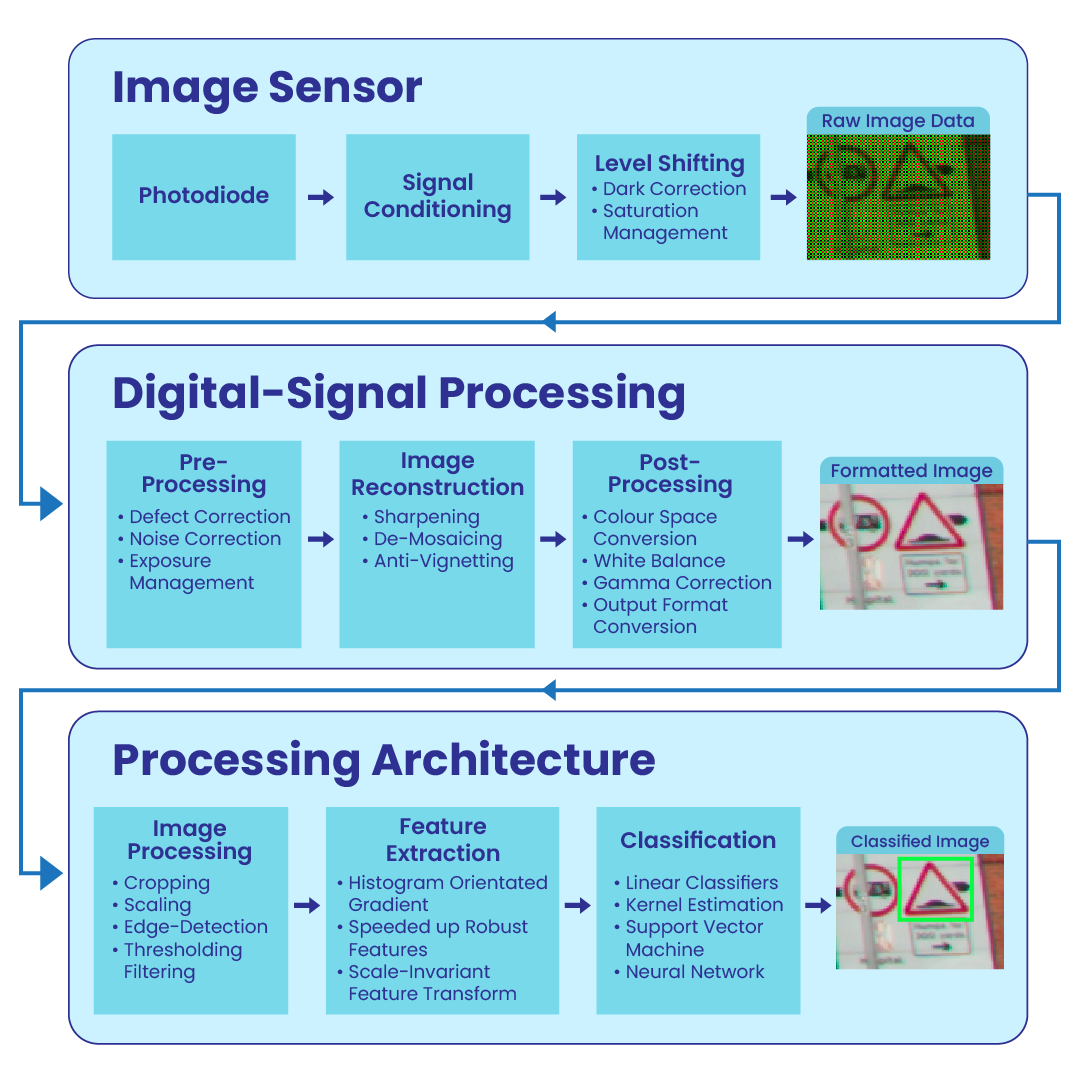
\includegraphics[width=\linewidth]{Images/vision_pipeline.png}
\caption[Image-Signal Pipeline]{Illustrates the key stages in processing an image signal, which includes the image sensor responsible for capturing data, the Digital Signal Processor (DSP) for signal processing, and processing architecture used for further image understanding and labelling.}
\label{fig:VisionPipeline}
\end{figure*} 
 
Vision applications fundamentally contain a sequence of operations that form a pipeline shown in \Fig{VisionPipeline}. Firstly, the image sensor captures photons reflected off objects using micro-lens to refract the light into a matrix of wells containing circuits called pixels and the charge produced from the photodiode is converted to a voltage. Once the analogue signal from the image sensor is converted into a digital format, the image data goes through various pixel and frame operations to correct any defects found from the introduction of noise. Furthermore, a full-colour image is reconstructed from the raw frame using a demosaicing algorithm, which may differ depending on the filter pattern \eg{Bayer, X-Trans or EXR}. Optionally, the colour image can be compressed into a JPEG format to reduce file size for transmission. The image may contain helpful features that define particular objects, such as shape, colour or texture information. Feature extraction algorithms help identify these characteristics and compile the features into a vector. Finally, a feature vector or image is inputted into a classification algorithm such as a convolution neural network to determine a label or 'class'. The sequence of operations within the pipeline can be reordered or removed to fulfil particular design requirements. %However, minor changes to the vision pipeline, such as implementing new camera architectures, require considerable revaluation of the image processing pipeline.

The imaging pipeline comprises various hardware and software components that enable the efficient implementation and execution of image processing algorithms. This chapter presents a complete overview of each component and its limitations. These components include imaging sensors, processing architectures, interface protocols, vision libraries and other tool-sets used to develop a heterogeneous system. 


%---------------------------------------------------------
\section{Imaging Sensor}
%---------------------------------------------------------
\begin{figure}[!t]
    \centering
    \begin{tabular}{cc}
    \resizebox{0.45\linewidth}{!}{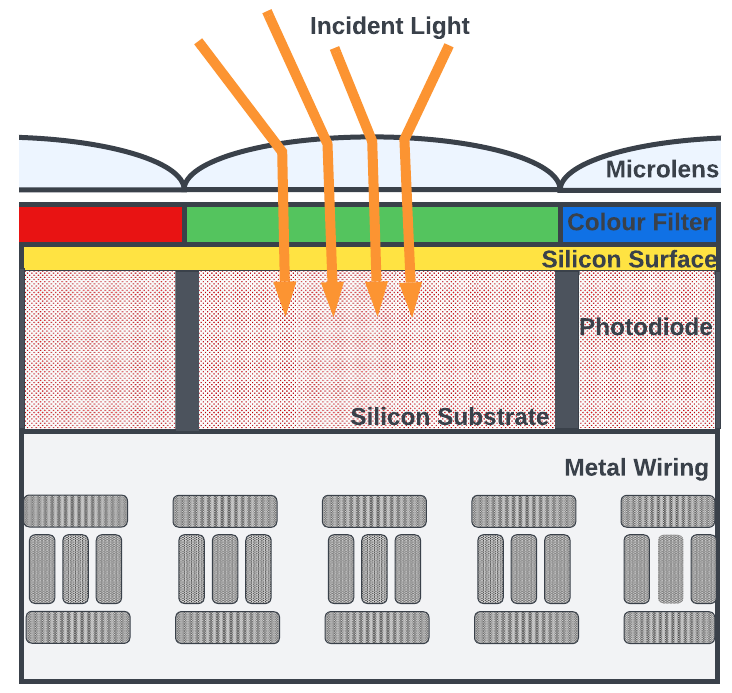
\includegraphics{Images/CMOSCrossSection.png}} &
    \resizebox{0.45\linewidth}{!}{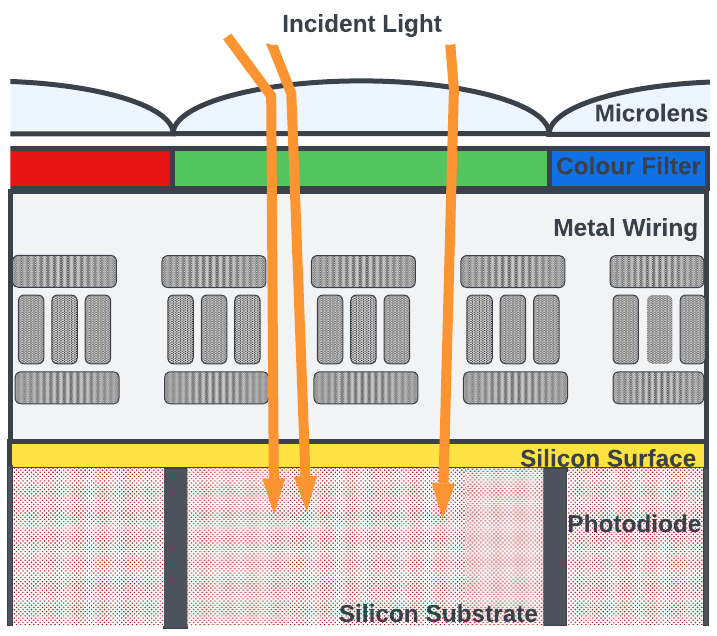
\includegraphics{Images/CMOSFI.png}} \\
    (a) Back-Illuminated & (b) Front-Illuminated \\
    \end{tabular}
    \caption[Image Sensor Architecture]{Cross-Section of CCD and CMOS silicon, revealing internal components fundamental to converting light into a signal.}
    \label{fig:CMOSCROSS}
\end{figure}


Image sensors are essential components in modern digital imaging devices, such as digital cameras, smartphones, and surveillance systems. These sensors play a crucial role in capturing and converting light into electrical signals, which are then processed to form digital images. Image sensors work on the principle of detecting and measuring light intensity to create a representation of the scene being captured. The most commonly used image sensing technologies within vision systems are charge-coupled device (CCD)\cite{Smi09}, and CMOS image sensor(CIS)\cite{Fos97}. CCD technology was developed first and optimised over time for imaging applications, which allowed it to gain a significant market share compared to the newly developed CIS technology, which suffered in image quality due to higher noise. Therefore, CIS sensors were only used in applications where lower cost was the driving factor over image quality. However, over the years, significant advances in silicon size, power consumption, process technology and the reduced fabrication cost of CIS technology resulted in surpassing CCD in market volume. CIS technology can now be found in many applications, from smartphones to medical imaging. Current research on CIS technology focuses on image quality by improving spatial, intensity, spectral and temporal characteristics \cite{Gou16}.

Modern image sensors comprise several layers shown in  \Fig{CMOSCROSS} that integrate together to capture and process light. At the topmost layer, microlenses focus incoming light onto the pixel array below, enhancing light sensitivity and overall image quality. Beneath the microlenses lies the pixel array, with each pixel containing a photodiode responsible for converting photons into electric charge. A Bayer pattern colour filter\cite{BayerPatent}, located on top of the pixel array, captures colour information by using red, green, and blue colour filters arranged in a specific pattern. Interpolating algorithms reconstruct the full-colour image from the captured colour data. Wiring and interconnects within the sensor facilitate the efficient transfer of electrical signals from each pixel to the readout circuitry, minimising signal degradation and cross-talk. The silicon substrate forms the foundation for all components, enabling efficient light conversion by the photodiodes and hosting the CMOS circuits for signal processing and readout. 



\begin{figure*}[!t]
    \centering
    \begin{tabular}{cc}
    \resizebox{0.48\linewidth}{!}{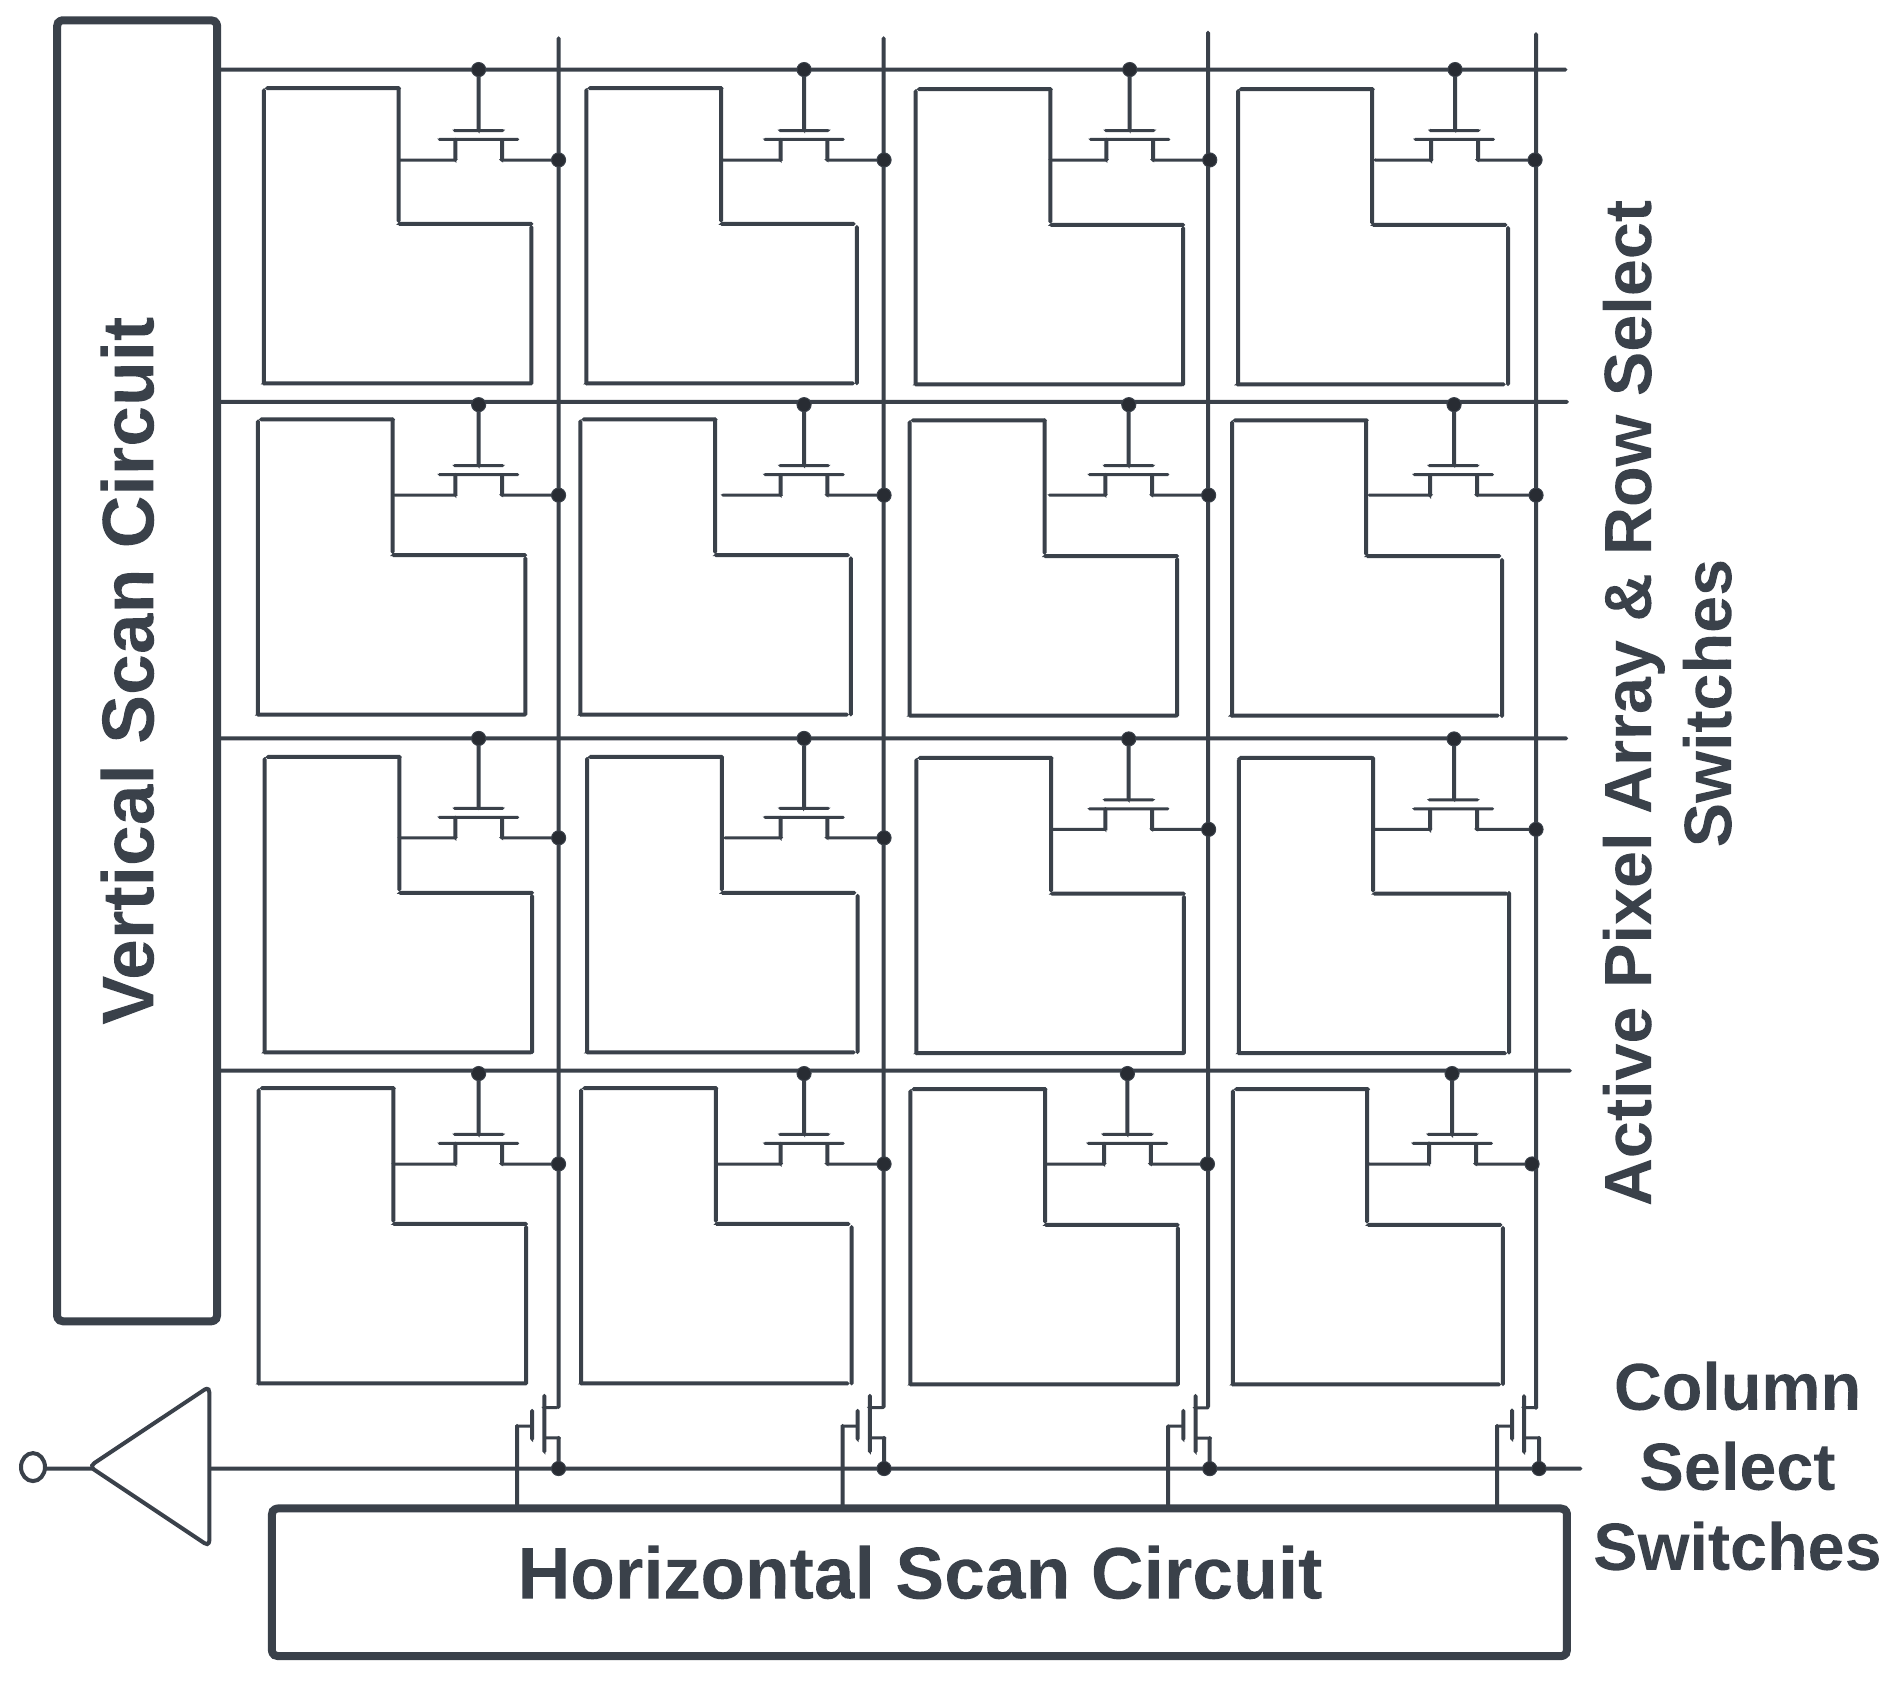
\includegraphics{Images/CMOS.png}} &
    \resizebox{0.5\linewidth}{!}{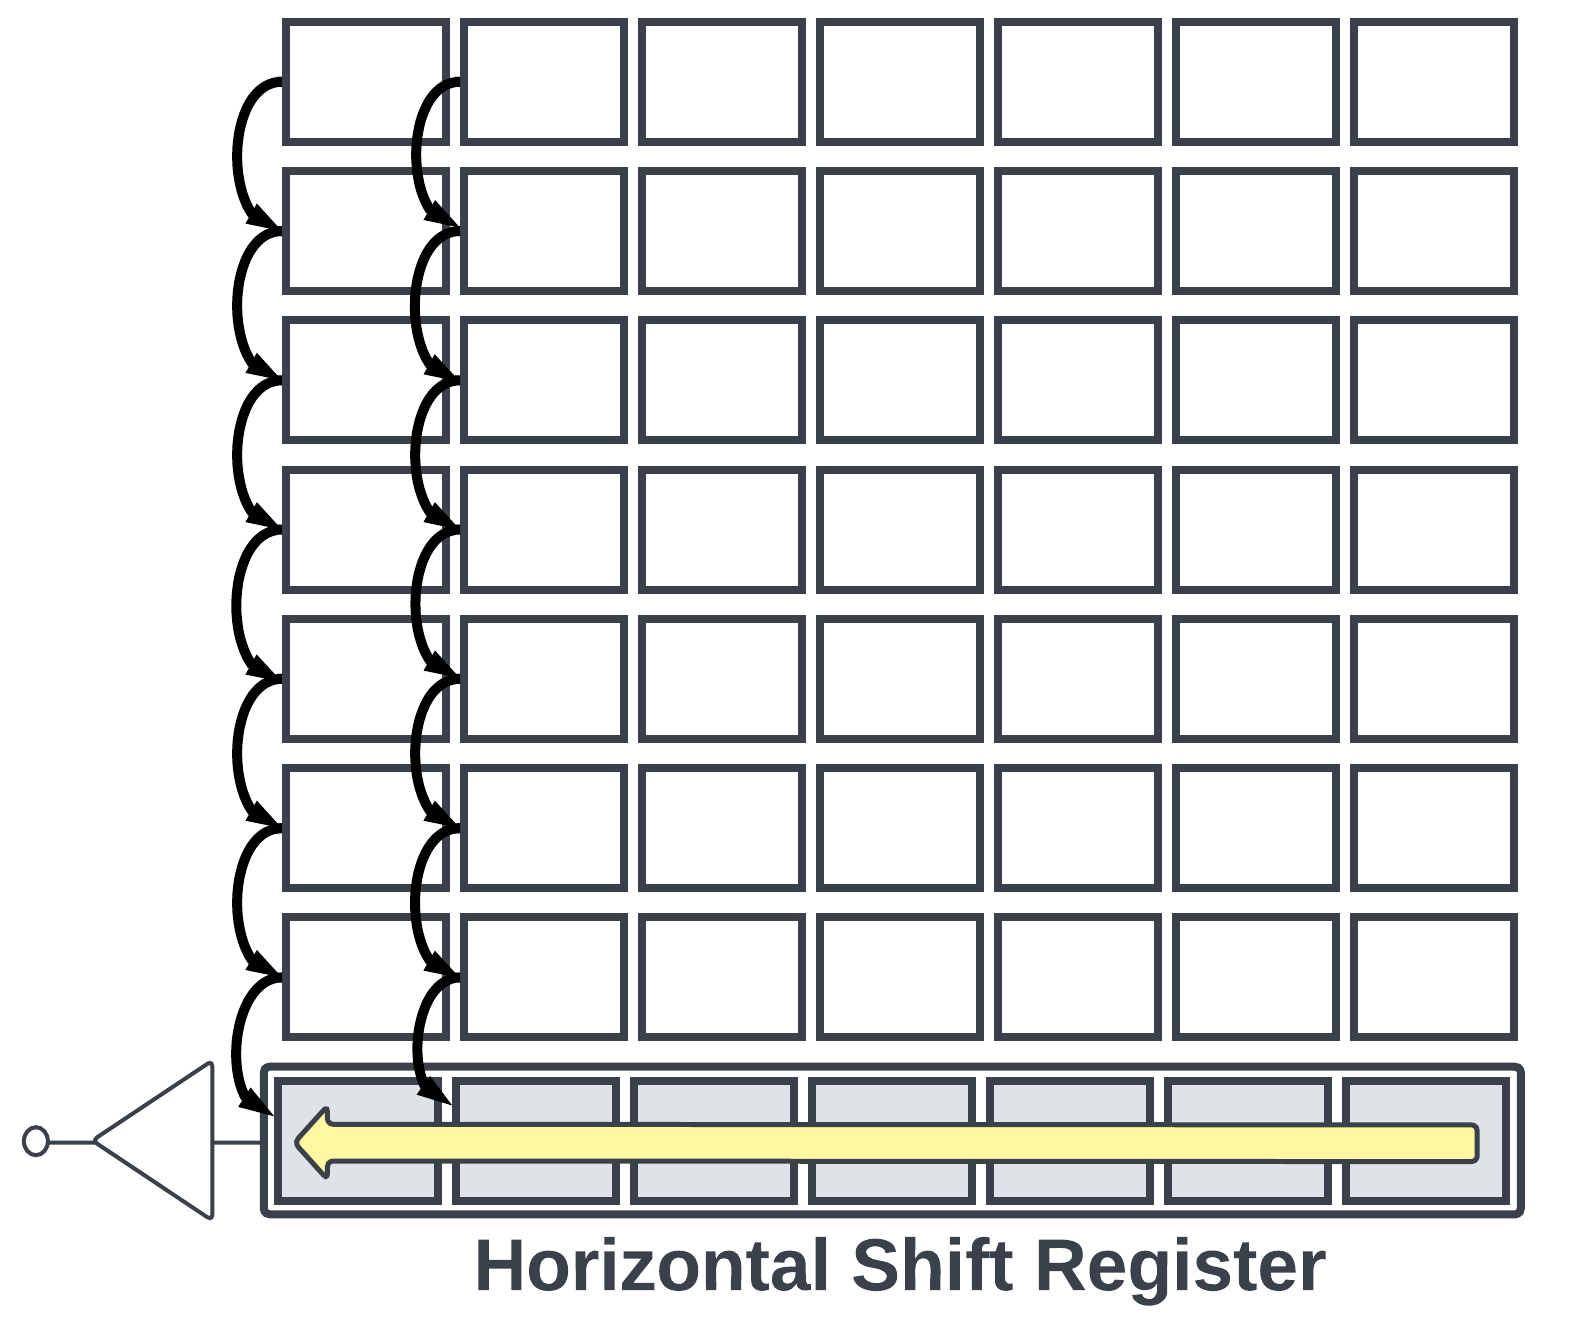
\includegraphics{Images/CCD.png}} \\
    (a) & (b) \\
    \end{tabular}
    \caption[Image Sensor Circuit Design]{a) CMOS Circuit  b) CCD Circuit, }
    \label{fig:CMOS Image Sensor}
\end{figure*}

The \textit{CCD} architecture operates on the principle of transferring charge thro-ugh a sequential shift register. This shift register is a critical component within the CCD chip, responsible for transporting the accumulated charge from each pixel to the output node for further processing. The photons of light strike the pixels of the CCD sensor, which absorbs the incident light, generating an electrical charge proportional to the intensity of the light. The charge in each pixel is horizontally transferred to neighbouring pixels along the shift register. This process, known as "horizontal transfer" in the row direction, uses potential wells to transport charge from one well to the next. After the horizontal transfer, the charge is vertically shifted down the columns. Manipulating voltages in the vertical shift registers moves the charge from one row to the next, guiding it towards the output node. The output node stores the accumulated charge and is connected to an analogue-to-digital converter (ADC) to convert the analogue charge into a digital signal for further processing and storage.

In a \textit{CMOS} image sensor, the conversion of light into voltage involves several technical steps. Each pixel in the sensor consists of a photodiode, which acts as a light-sensitive capacitor. When incident photons strike the photodiode, it generates electron-hole pairs, and these charge carriers are stored as electric charge in the capacitor. The accumulated charge in each pixel's capacitor is then transferred to an associated charge-to-voltage conversion circuit, commonly known as the readout circuit. This circuit typically includes a source follower amplifier or a trans-impedance amplifier. The charge is converted into a corresponding analogue voltage signal, proportional to the intensity of the incident light on the pixel. The output voltage from each pixel is then sent to the image sensor's output circuitry for further signal conditioning and processing. This circuitry may include analogue signal processing components such as analogue filters or amplifiers to enhance the image quality and reduce noise.

\begin{figure*}[!t]
    \centering
    \begin{tabular}{cc}
    \resizebox{0.46\linewidth}{!}{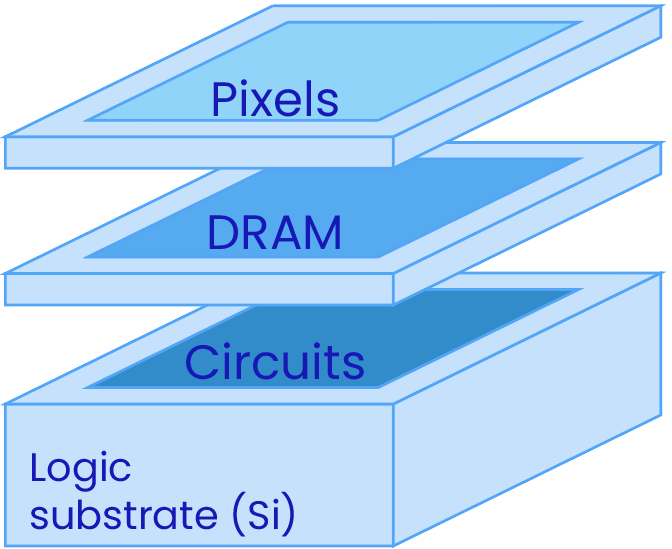
\includegraphics{Images/3dstack.png}} &
    \resizebox{0.46\linewidth}{!}{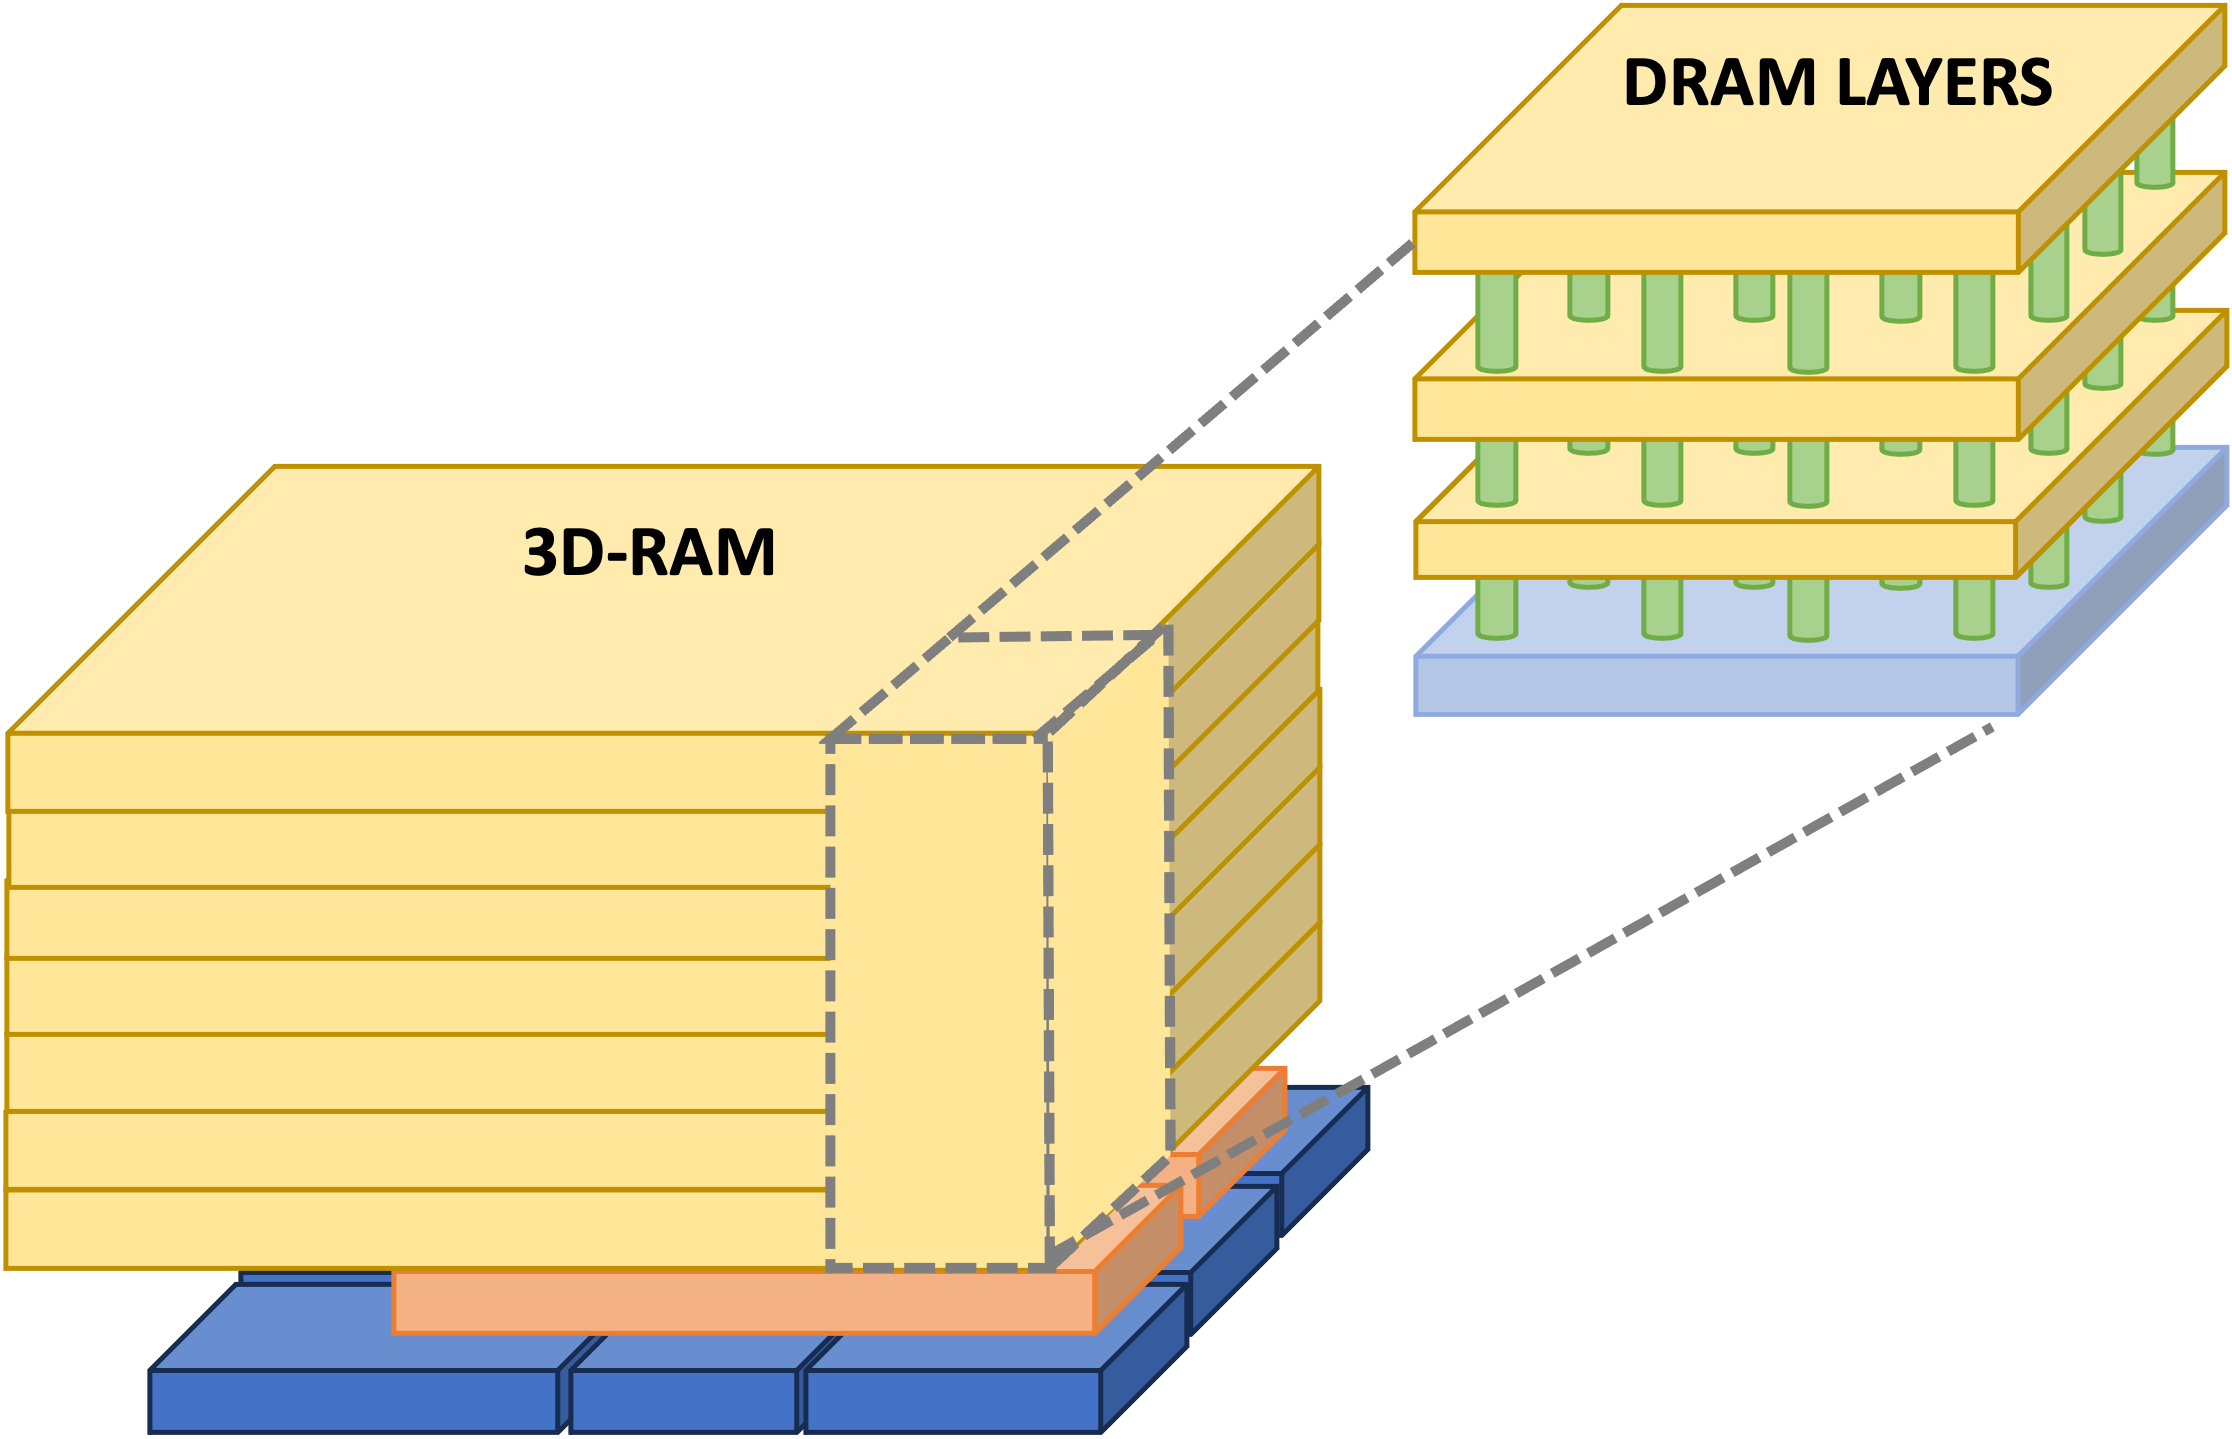
\includegraphics{Images/memorystack.png}} \\
    (a) & (b) \\
    \end{tabular}
    \caption[3D Stacked Image Sensor and Memory ]{a) 3D Stacked Image Sensor b) 3D Stacked Memory; The Configuration Employs Multiple Processing or Memory Layers Vertically Stacked on Top of Each Other, Linked by Through-Silicon Vias (TSVs) and Microbumps. }
    \label{fig:3DStacking}
\end{figure*}


In machine vision, the key performance metrics are latency and noise. The differences arise between CMOS and CCD imagers in their signal conversion processes, transitioning from signal charge to an analogue signal and finally to a digital one. In CMOS area and line scan imagers, a highly parallel front-end design enables low bandwidth for each amplifier. Consequently, when the signal encounters the data path bottleneck, typically at the interface between the imager and off-chip circuitry, CMOS data firmly resides in the digital domain. Conversely, high-speed CCDs possess numerous parallel fast output channels, albeit not as massively parallel as high-speed CMOS imagers. As a result, each CCD amplifier requires higher bandwidth, leading to increased noise levels. Therefore, high-speed CMOS imagers exhibit the potential for considerably lower noise compared to high-speed CCDs.

In recent years, semiconductor manufacturers have moved onto stacking imaging sensors depicted in \Fig{3DStacking} to reduce the latency between readout to processing, which was previously developed in the memory domain to increase data storage. 


\subsection{Image Sensor Characterisation}
\begin{figure}[!t]
\centering
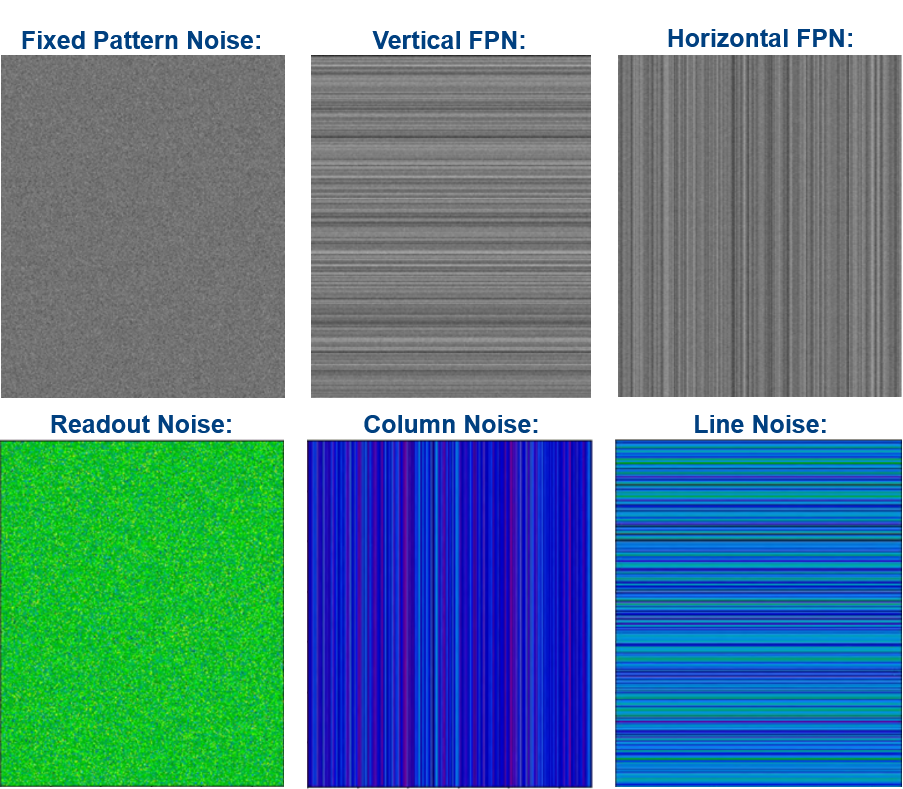
\includegraphics[width=\linewidth]{Images/FixedPatternNoise.png}
\caption[Image Sensor Noises]{The figure illustrates the presence of characteristic fixed noise patterns, often resulting from sensor imperfections or calibration issues, alongside temporal noise, which can manifest as random variations in pixel values over multiple frames.}
\label{fig:NoiseyImage}
\end{figure} 

Image sensor characterisation is a process that assesses the performance and capabilities of imaging sensors. The goal is to understand the sensor's behaviour and limitations to ensure optimal image quality and accurate representation of the captured scene. Noise introduced in sensors come from various sources such as thermal noise, read noise, and photon shot noise, which can degrade image quality, as observed in \ref{fig:NoiseyImage}. Characterisation involves measuring and analysing these noise components to determine their impact on image fidelity. Noise can be separated into two categories:

\begin{itemize}
  \item \textbf{Pattern Noise:}
  \par
  This term describes noise patterns that remain constant or fixed over time and across multiple frames or exposures. Fixed pattern noise includes phenomena like Fixed Pattern Noise (FPN), Pixel Non-Uniformity (PRNU), and other systematic and deterministic noise sources.

  \item \textbf{Random Noise:}
  \par
  The random noise relates to noise that varies over time or across different exposures. It includes sources of noise that exhibit randomness and unpredictability from frame to frame, such as Photon Shot Noise, Readout Noise, Amplifier Noise, and Jitter Noise.
\end{itemize}

Signal-to-noise ratio (SNR) is a standard metric used to quantify the signal quality captured by the sensor relative to the noise in the image. Dynamic range is another parameter that refers to the sensor's ability to capture and distinguish details in a scene's bright and dark regions. A wide dynamic range is essential for preserving details in high contrast scenes without overexposing or underexposing certain areas. Sensitivity and linearity are additional metrics assessed during the characterisation process. Sensitivity determines how well the sensor responds to incoming light, while linearity examines how the sensor's output corresponds to the actual incident light levels.



%--------------------------------------------------------
\section{Interface Technologies}
Vision systems typically rely on input from cameras or other video sources, generating a continuous stream of image frames. Designing algorithms for embedded vision systems requires a detailed understanding of performance and interfacing technologies. The subsequent sections provide an overview of various characteristics related to each technology.

\subsection{Camera Link}
\begin{figure}[!h]
\centering
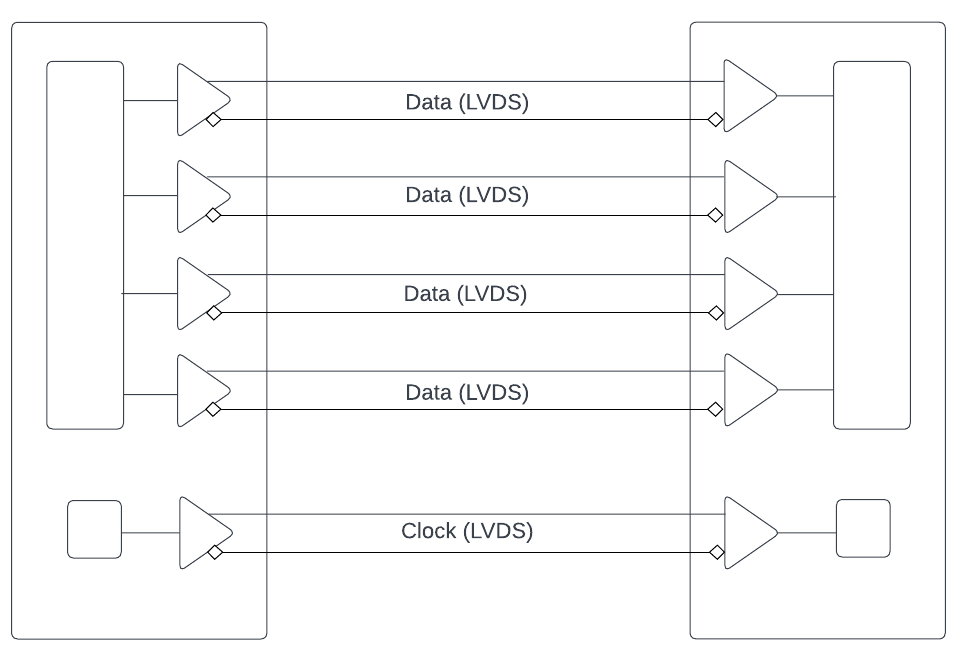
\includegraphics[width=0.7\linewidth]{Images/CameraLink.png}
\caption[Camera Link Architecture]{Camera Link interface, showing the integration of Low Voltage Differential Signalling (LVDS) technology for noise immunity.}
\label{fig:CameraLink}
\end{figure} 

Camera Link\cite{CameraLink} is a parallel communication protocol that extends the Channel Link technology and standardises the interface between cameras and frame grabbers. Channel Link provides a one-way transmission of 28 data signals and an associated clock over five LVDS pairs. Among these pairs, one is designated for the clock, while the 28 data signals are multiplexed across the remaining four pairs exhibited in \Fig{CameraLink}, involving a 7:1 serialisation of the input data. A single Camera Link connection allocates 24 bits for pixel data (three 8-bit pixels or two 12-bit pixels) and reserves 4 bits for frame, line, and pixel data valid signals. The pixel clock operates at a maximum rate of 85 MHz. Additionally, four LVDS pairs facilitate general-purpose camera control from the frame grabber to the camera, with the specifics defined by the camera manufacturer. Furthermore, two LVDS pairs are designated for asynchronous serial communication between the camera and frame grabber, supporting a minimum baud rate of 9600 for relatively low-speed serial communication.

For higher bandwidth requirements, the medium configuration includes an additional Channel Link connection, granting an extra 24 bits of pixel data. The full configuration further extends the capacity by incorporating a third Channel Link, resulting in a total of 64 bits of pixel data transmission capability. The versatile nature of Camera Link, with its various configurations, makes it a widely adopted interface standard for high-performance camera systems, particularly in applications demanding real-time image capture and processing.






\subsection{Peripheral Component Interface Express (PCIe)}
\begin{figure}[!h]
\centering
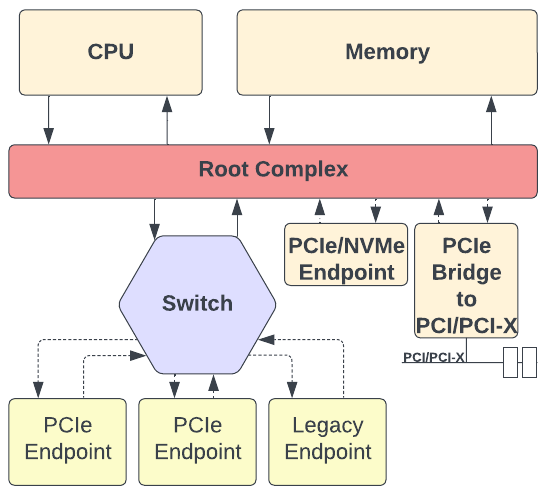
\includegraphics[width=0.6\linewidth]{Images/PCIe.png}
\caption[PCIe Architecture]{The PCIe Architecture consists of Root Complex, PCIe Endpoint Devices, and Memory Subsystem. The Root Complex orchestrates data flow, while PCIe Endpoint Devices serve as endpoints for data transactions.}
\label{fig:PCIe}
\end{figure} 


The Peripheral Component Interface Express (PCIe)\cite{PCIe} shown in \Fig{PCIe}, is an open standard serial bus interface protocol designed in the early 1990s to provide a high-speed interconnect between devices such as Ethernet controllers, expansion/capture cards, storage and graphics processing units. The protocol defined a set of registers within each device known as configuration space, allowing software to view memory and IO resources. In addition, the exposure of peripheral data enables software to assign an address to each device without conflict with other systems. Table \ref{tab:PCIeSummary} summarises each version of the PCIe specification ratified in the past and future.


\begin{figure}[h]
\centering
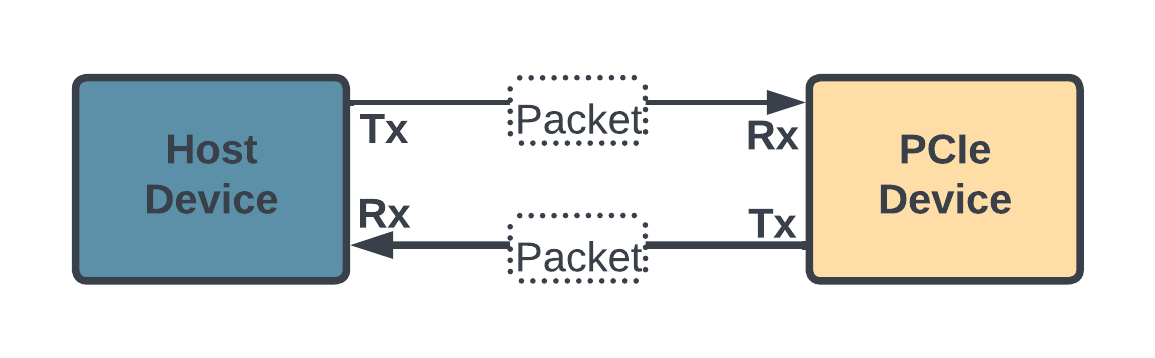
\includegraphics[width=0.9\linewidth]{Images/PCIELink.png}
\caption[PCIe Link]{The PCIe Communication Data Link between two Devices}
\label{fig:PCIeDualSimplexLink}
\end{figure} 


The PCIe architecture consists of a root complex that connects the CPU and memory subsystem to the PCI Express switch fabric composed of one or more PCIe/PCI endpoints. The dual‐simplex connections between endpoints are bidirectional, as shown in \Fig{PCIeDualSimplexLink}, which allows data to be transmitted and received simultaneously. The term for this path between the devices is a Link and is made up of one or
more transmit and receive pairs. One such pair is called a Lane, and the spec
allows a Link to be made up of 1, 2, 4, 8, 12, 16, or 32 Lanes. The number of lanes is
called the Link Width and is represented as x1, x2, x4, x8, x16, and x32. The trade‐off regarding the number of lanes to be used in a given design is that having more lanes increases the Link's bandwidth but at the cost of space requirement and power consumption.




\begin{table}[H]
\centering
\caption{PCIe Specification Summary.}
\label{tab:PCIeSummary}
\resizebox{\linewidth}{!}{%
\begin{tabular}{ccccc} 
\hline
\rowcolor[rgb]{0.753,0.753,0.753} \multicolumn{1}{c|}{\begin{tabular}[c]{@{}>{\cellcolor[rgb]{0.753,0.753,0.753}}c@{}}\textbf{PCIe}\\\textbf{ Specification}\end{tabular}} & \multicolumn{1}{c|}{\begin{tabular}[c]{@{}>{\cellcolor[rgb]{0.753,0.753,0.753}}c@{}}\textbf{Release}\\\textbf{ Year}\end{tabular}} & \multicolumn{1}{c|}{\begin{tabular}[c]{@{}>{\cellcolor[rgb]{0.753,0.753,0.753}}c@{}}\textbf{Data Rate }\\\textbf{ (GT/s)}\end{tabular}} & \multicolumn{1}{c|}{\textbf{Encoding}} & \begin{tabular}[c]{@{}>{\cellcolor[rgb]{0.753,0.753,0.753}}c@{}}\textbf{Total}\\\textbf{ Bandwidth (GB/s)}\end{tabular} \\ 
\hline
PCIe 1.0 & 2003 & 2.5 & 8b/10b & 8 \\
PCIe 2.0 & 2007 & 5 & 8b/10b & 16 \\
PCIe 3.0 & 2010 & 8 & 128b/130b & 32 \\
PCIe 4.0 & 2017 & 16 & 128b/130b & 64 \\
PCIe 5.0 & 2019 & 32 & 128b/130b & 128 \\
PCIe 6.0 & 2021 & 64 & PAM-4/FLIT & 256 \\
PCIe 7.0 & 2023 & 128 & PAM-16/FLIT & 512 \\
\hline
\end{tabular}
}
\end{table}



%====================================

\subsection{Ethernet}
Ethernet technology\cite{Ethernet} is based on the Carrier Sense Multiple Access with Collision Detection (CSMA/CD) access method. It operates at the physical layer (Layer 1) and the data link layer (Layer 2) of the OSI model. The physical layer handles the transmission and reception of raw data over the physical medium, while the data link layer is responsible for framing, addressing, and error detection.

One of the main advantages of Ethernet is its flexibility and scalability. It can support various data rates, ranging from 10 Mbps for older versions (e.g., 10BASE-T) to 1 Gbps (Gigabit Ethernet) and beyond for modern implementations. This adaptability allows Ethernet to cater to a wide range of applications, from simple office networks to high-speed data centres and multimedia streaming.

When using Ethernet with FPGAs, designers face the challenge of implementing the higher layers of the OSI model, namely the network layer (Layer 3) and transport layer (Layer 4). These layers are responsible for IP addressing, routing, and end-to-end communication. FPGA designs must include logic to handle IP addressing, packet forwarding, and any higher-level protocols required for data exchange. This complexity can add overhead to the FPGA design and require careful optimisation to ensure efficient data processing.

In FPGA-based systems, the communication between the FPGA and the Ethernet physical layer typically involves a Media Access Control (MAC) core, which is responsible for generating and interpreting Ethernet frames. The MAC core interfaces with the external Ethernet PHY chip, which handles the conversion between the MAC-level signals and the actual physical signals transmitted over the Ethernet cable. In CPU-based systems, handling Ethernet involves the integration of a Network Interface Controller (NIC) or Ethernet controller. The NIC is a hardware component that interfaces the CPU with the Ethernet medium. It manages low-level operations, such as frame reception and transmission, packet encapsulation and decapsulation, and error checking. The NIC communicates with the CPU through driver software that implements higher-level network protocols.

The CPU's involvement in Ethernet communication extends beyond the data link layer. It handles the network layer protocols (Layer 3), such as Internet Protocol (IP), which involves tasks like IP address assignment, routing, and packet forwarding. Additionally, the CPU manages transport layer protocols (Layer 4), such as Transmission Control Protocol (TCP) and User Datagram Protocol (UDP), responsible for end-to-end communication and data flow control. 

\subsubsection{GigE Vision}
\begin{figure}[H]
\centering
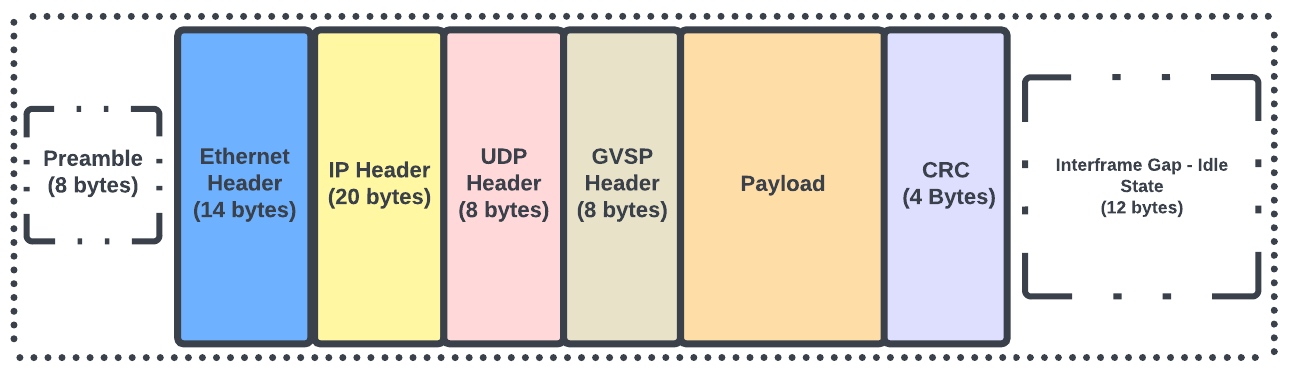
\includegraphics[width=\linewidth]{Images/GigEVision.png}
\caption[GigE Vision Stream Packet]{A Structure of the Data Frame, Including Payload Data, Header Information, and Ethernet Protocol Stack.}
\label{fig:GigEVision}
\end{figure} 

GigE Vision is a standard developed in 2006 by the Automated Imaging Association\cite{GigE}, which extends gigabit Ethernet to transport video data and control information to the camera efficiently. This standard benefits from the widespread availability of low-cost standard cables and connectors, allowing data transfer rates of up to 100 MPixels per second over distances of up to 100 meters.

GigE Vision comprises four essential elements. The control protocol facilitates camera control and configuration communication, while the stream protocol governs the transfer of image data from the camera to the host system, both running over UDP. A device discovery mechanism identifies connected GigE Vision devices and acquires their internet addresses. GigE Vision utilises Gigabit Ethernet (1000BASE-T) for data transmission, enabling a maximum data rate of 1 Gbps for real-time transfer of large image and video data in industrial applications. It employs packet-based communication displayed in \Fig{GigEVision}, dividing images into smaller packets for efficient data transfer, ensuring reliable transmission and minimal data loss. Moreover, many GigE Vision cameras support Power over Ethernet (PoE), receiving power through the Ethernet cable, reducing installation overhead. 
GigE Vision supports both asynchronous and synchronous triggers for precise image capture control. Asynchronous triggers allow continuous image capture at a specified frame rate, while synchronous triggers enable coordinated capture based on external events for synchronised operation with other devices. Additionally, GigE Vision cameras can be easily configured and accessed using the GigE Vision Control Protocol (GVCP), providing efficient camera parameter adjustments and image data retrieval. Overall, GigE Vision is a versatile and efficient interface for industrial imaging applications, offering seamless data transmission and easy camera control.

In many embedded vision applications, it is more practical to integrate the FPGA system within the camera itself, allowing for image processing before transmitting results to a host system using GigE Vision. To achieve real-time operation, a dedicated device driver is used on the host system. This driver bypasses the standard TCP/IP protocol stack for the video stream and employs Direct Memory Access (DMA) transfers to transfer data to the application directly. By avoiding CPU overhead during video data handling, real-time performance can be achieved effectively. This optimised data transfer scheme ensures smooth and efficient communication between the camera and the host system in GigE Vision applications.



\subsection{Universal Serial Bus (USB)}
\begin{table}[tb]
\centering
\caption{USB Versions, Bandwidth, Power Supply, and Specifications.}
\label{tab:usb_versions}
\resizebox{\linewidth}{!}{%
\begin{tabular}{cccc} 
\hline
\rowcolor[rgb]{0.753,0.753,0.753} \multicolumn{1}{c|}{\textbf{USB Version}} & \multicolumn{1}{c|}{\textbf{Bandwidth}} & \multicolumn{1}{c|}{\textbf{Power Supply}} & \textbf{Additional Information} \\ 
\hline
USB 1.0 & 1.5 Mb/s & 5V (Max 500mA) & Initial USB standard \\
USB 1.1 & 12 Mb/s & 5V (Max 500mA) & Enhanced data rate \\
USB 2.0 & 480 Mb/s & 5V (Max 500mA) & High-speed data transfer \\
USB 3.0 & 5 Gb/s & 5V (Max 900mA) & SuperSpeed USB \\
USB 3.1 & 10 Gb/s & 5V (Max 900mA) & SuperSpeed+ USB \\
USB 3.2 & 20 Gb/s & 5V (Max 900mA) & SuperSpeed USB 10, 20 Gb/s \\
USB 4.0 & 40 Gb/s & 5V (Max 900mA) & Thunderbolt 3 compatible \\
\hline
\end{tabular}
}
\end{table}
USB has emerged as a widely used interface for connecting peripheral devices to personal computers. Over the years, USB technology has evolved significantly, supporting increasing link speeds from the initial 1.5 Mb/s and 12 Mb/s to the current 20 Gb/s in the double lane configuration of USB 3.2 Gen 2. As a result, USB has proven to be a viable and versatile interface between FPGAs and SoCs (System-on-Chips) in various applications.

USB operates in a master-slave architecture, where there can be only one host or master controller within a USB network, and the host controller initiates all communication. The communication protocol of USB is structured into four layers: the application and system software interacts with the USB pipe at the topmost layer, while the protocol layer handles packet management. USB packets come in several types, such as Link Management Packets, Transaction Packets, Data Packets, and Isochronous Timestamp Packets. These packets serve to exchange control and status information between the host and the connected devices.

The Data Packet, which carries user data along with a 16-byte header, is essential for transferring information between the host and the device. On the other hand, the other packet types primarily facilitate control and status exchanges. Any data transfer requires initiation by a Transaction Packet before actual data transmission occurs. To enable FPGA access to the USB bus, an external PHY (Physical Layer) chip is necessary. This chip often provides a first-in-first-out (FIFO) interface, which the FPGA can connect to through regular I/O ports. User logic is then required to implement the control logic and interface with the application. While this FIFO interface might limit throughput in certain scenarios, it does not pose any bottleneck for applications like video streaming. 


%--------------------------------------------------------



\subsection{Mobile Industry Processor Interface (MIPI)}

\begin{figure}[!h]
\centering
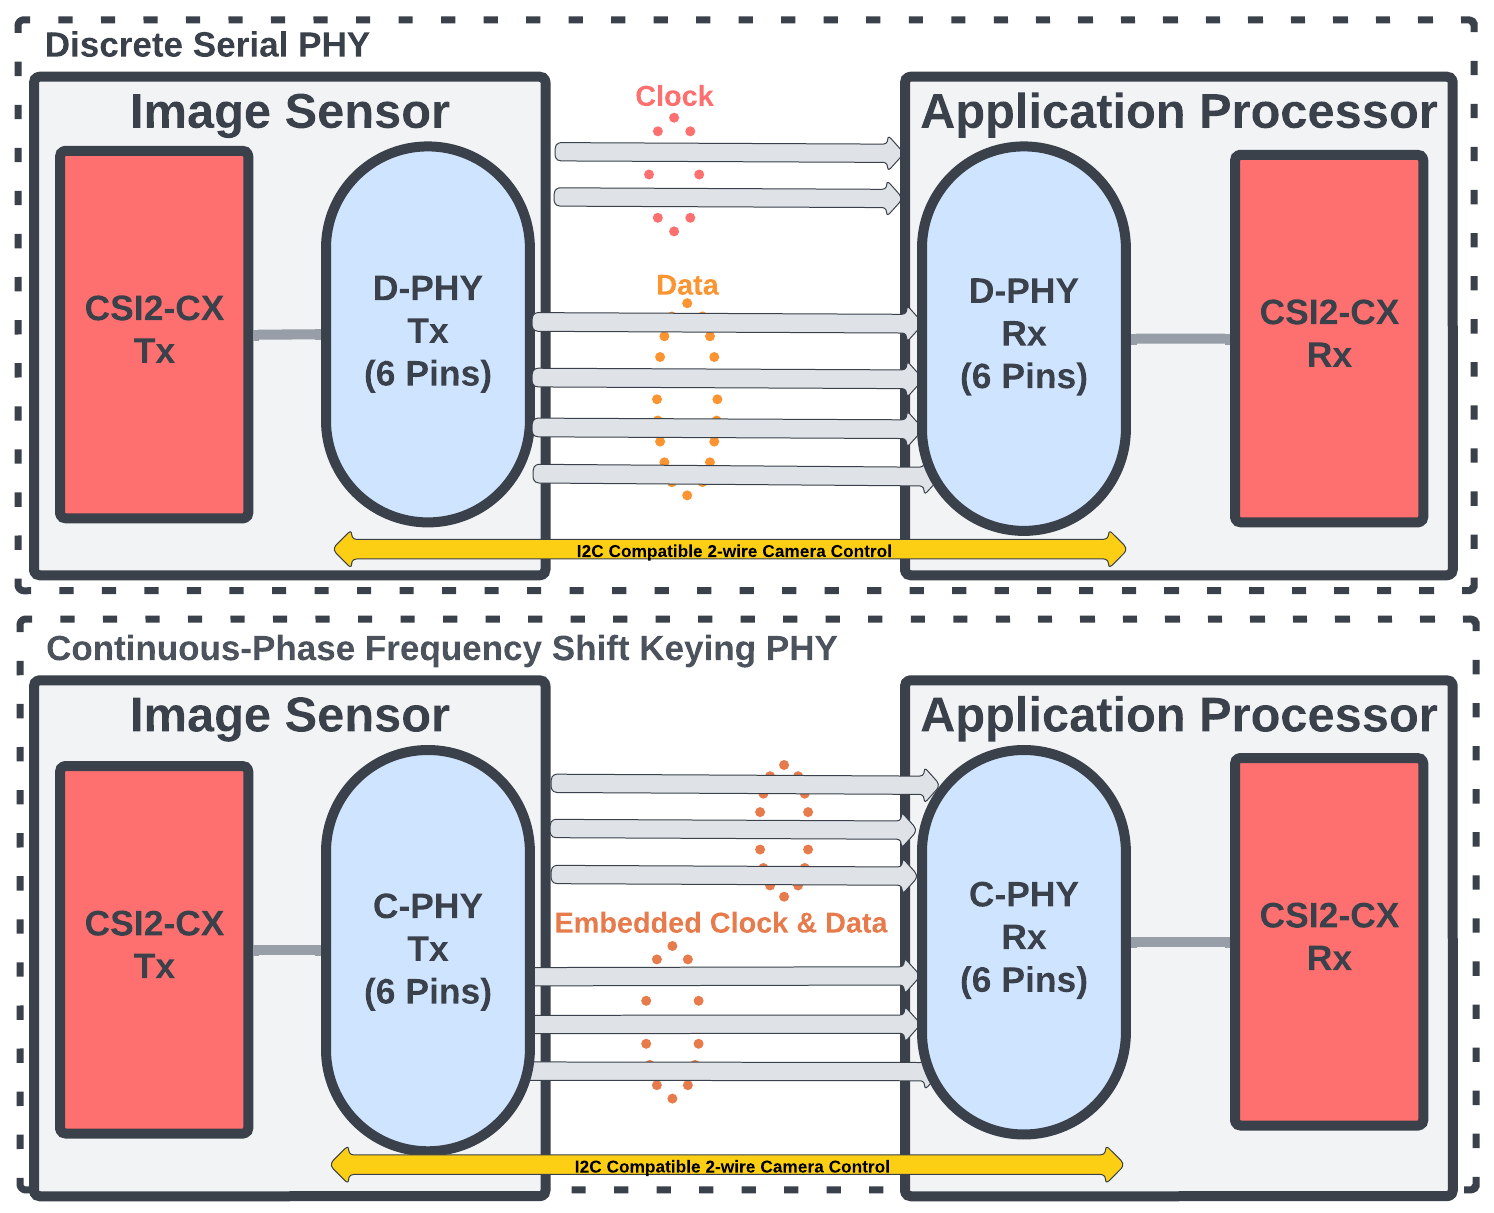
\includegraphics[width=0.7\linewidth]{Images/MIPI.png}
\caption[MIPI Architecture]{C-PHY and D-PHY with two lanes each. C-PHY makes it possible to reach more than double the bandwidth per lane than D-PHY.}
\label{fig:MIPI}
\end{figure} 


MIPI\cite{mipi} is a serial interface standard developed in 2003 for interconnecting components in mobile devices. MIPI comes in various versions, and one of the widely used versions in mobile camera interfaces is MIPI CSI-2 (Camera Serial Interface 2). The interface can consist of one or more data lanes, each capable of transmitting a stream of image data. A separate clock lane synchronises the data transmission, ensuring accurate data reception. MIPI CSI-2 supports various data types, including RAW image data and metadata, allowing it to accommodate different image sensor formats and data requirements. Furthermore, the concept of virtual channels enables the multiplexing of multiple data types over the same physical data lanes.

MIPI CSI-2 utilises low-voltage differential signalling to transmit image data from the camera sensor to the application processor. C-PHY and D-PHY are two different physical layer specifications, and their usage depends on the specific requirements of the devices shown in \Fig{MIPI}. D-PHY provides higher data rates and is capable of reaching extremely high speeds, making it suitable for applications that require substantial data throughput. D-PHY supports multiple data lanes (typically 1 to 4 lanes), and it is commonly used in devices with high-resolution imaging requirements, such as high-end smartphones and cameras. On the other hand, C-PHY, or Combo PHY, is a combination of MIPI C-PHY and MIPI D-PHY technologies. It offers a more power-efficient solution than D-PHY, making it ideal for power-sensitive mobile devices. C-PHY leverages both a low-power, single-ended signalling mode and a high-speed, differential signalling mode, providing a balance between data transfer rates and power consumption. It uses fewer wires compared to D-PHY, simplifying the physical design of mobile devices and potentially reducing costs.

MIPI CSI-2 comes with certain drawbacks that may impact its applicability. Firstly, its physical image data transfer (D-PHY) is limited to shorter cable lengths, typically not exceeding 20 cm, which can be restrictive for certain industrial applications. Additionally, the lack of a standardised plug for MIPI CSI-2 means that sensor/camera modules must be individually and proprietary connected. Moreover, the absence of a standardised driver and software stack requires custom adjustments for each sensor or camera module to work with the CSI-2 driver of a specific System-on-Chip (SoC) through a proprietary I²C driver as a Video4Linux sub-device.  

\subsection{FPGA Mezzanine Card (FMC)}
\begin{figure}[h]
\centering
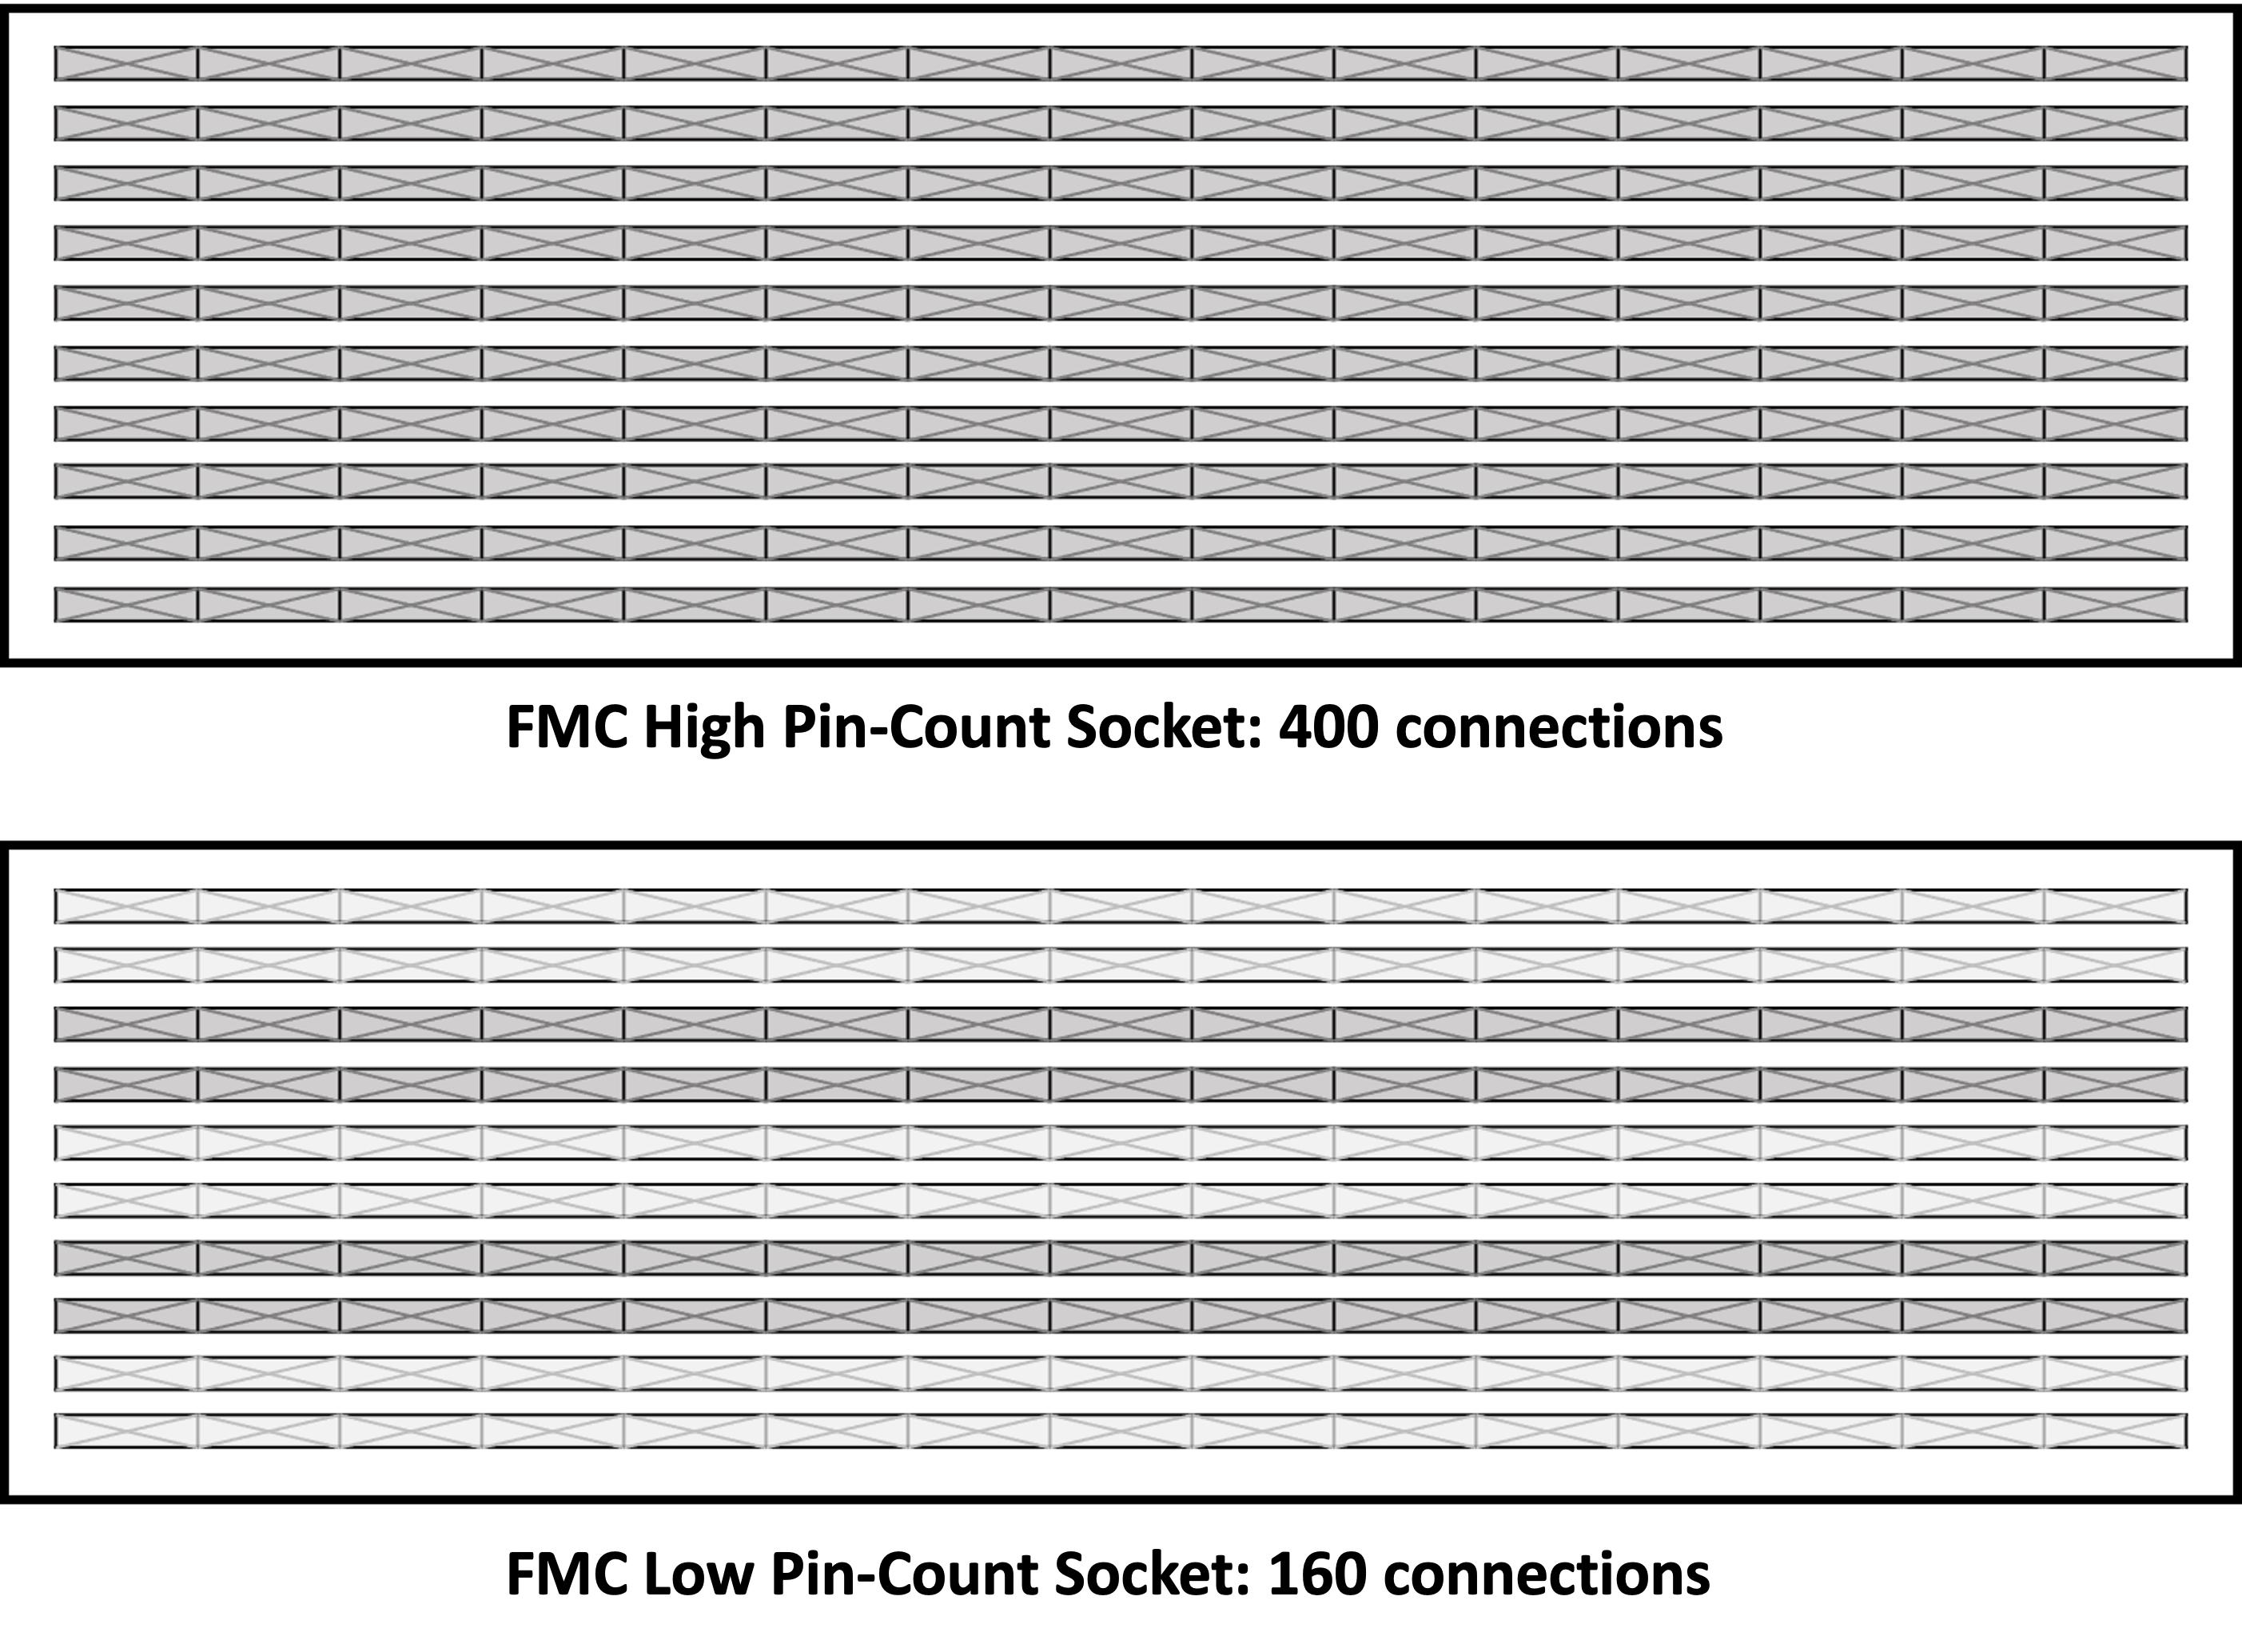
\includegraphics[width=0.7\linewidth]{Images/FMCPincount.png}
\caption[FMC Architecture]{FMC Low Pin and High Pin Count Sockets.}
\label{fig:FMC}
\end{figure} 

The FMC interface is a high-speed, versatile standard for connecting external modules to FPGAs (Field-Programmable Gate Arrays). The FMC standard encompasses two form factors: single-width and double-width. Single-width supports one connector, while double-width caters to applications needing more bandwidth, front panel space, or larger PCB areas and supports up to two connectors, offering designers flexibility for optimising space and I/O requirements. Two connector types, Low Pin Count (LPC) with 160 pins and High Pin Count (HPC) with 400 pins, displayed in \Fig{FMC}. Both support single-ended and differential signalling up to 2 Gb/s, with signalling to an FPGA's serial connector at up to 10 Gb/s. LPC offers 68 user-defined single-ended signals or 34 differential pairs, along with clocks, a JTAG interface, and optional I2C support for base Intelligent Platform Management Interface (IPMI) commands. HPC provides 160 single-ended signals (or 80 differential pairs), ten serial transceiver pairs, and additional clocks. HPC and LPC connectors use the same mechanical connector, differing only in populated signals, enabling compatibility between them.

%It features a compact, rugged form factor that ensures robust connectivity while supporting a wide range of data rates and interfaces. FMC modules typically consist of high-speed serial transceivers, I/O pins, and interface connectors, allowing for seamless integration of specialised functionalities such as analogue-to-digital conversion, memory storage, or custom interfaces with FPGA-based systems. 




\subsection{Summary}
\begin{table}[H]
\centering
\caption{Image Sensor Interfaces Specifications.}
\label{tab:Interfaces}
\resizebox{\linewidth}{!}{%
\begin{tabular}{ccccccc} 
\hline
\rowcolor[rgb]{0.753,0.753,0.753} \multicolumn{1}{c|}{\textbf{Interface}} & \multicolumn{1}{c|}{\begin{tabular}[c]{@{}>{\cellcolor[rgb]{0.753,0.753,0.753}}c@{}}\textbf{Interface }\\\textbf{ Type}\end{tabular}} & \multicolumn{1}{c|}{\textbf{Bandwidth}} & \multicolumn{1}{c|}{\begin{tabular}[c]{@{}>{\cellcolor[rgb]{0.753,0.753,0.753}}c@{}}\textbf{Max Cable}\\\textbf{ Length}\end{tabular}} & \multicolumn{1}{c|}{\begin{tabular}[c]{@{}>{\cellcolor[rgb]{0.753,0.753,0.753}}c@{}}\textbf{Max}\\\textbf{Frequency}\end{tabular}} & \multicolumn{1}{c|}{\begin{tabular}[c]{@{}>{\cellcolor[rgb]{0.753,0.753,0.753}}c@{}}\textbf{Bit}\\\textbf{ Depth}\end{tabular}} & \begin{tabular}[c]{@{}>{\cellcolor[rgb]{0.753,0.753,0.753}}c@{}}\textbf{Power}\\\textbf{ (W)}\end{tabular} \\ 
\hline
PCIe & Serial & Up to 32 Gbps & 0.2 Metres & 100 MHz & Varies & 75 W \\
GigE Vision & Serial & Up to 1 Gbps & 100 Metres & 125 MHz & 8/10/12/14/16 bit & 12 W \\
Camera Link & Parallel & Up to 800 Mbps & 10 Metres & 85 MHz & 8/10/12/14 bit & 6 W \\
MIPI CSI-2 & Serial & Up to 10 Gbps & 0.2 Metres & 250 MHz & 8/10/12/14/16/24 bit & 1.2 W \\
FireWire & Serial & Up to 800 Mbps & 4.5 Metres & 400 MHz & 8/10 bit & 6 W \\
CoaXPress & Serial & Up to 12.5 Gbps & 100 Metres & 250 MHz & 8/10/12 bit & 24 W \\
USB4 & Serial & Up to 40 Gbps & 2 Metres & 100 MHz & 8-32 bit & 7.5 W \\
10 GigE & Serial & Up to 10 Gbps & 100 Metres & 156.25 MHz & 8/10/12/14 bit & 15 W \\
Thunderbolt 4 & Serial & Up to 40 Gbps & 3 Metres & 648.91 MHz & 8/10 bit & 9.9 W \\
FMC & Both & Up to 40 Gbps & 1 Metre & 156.25 MHz & 8/10/12/14/16 bit & 6.6 W \\
\hline
\end{tabular}
}
\end{table}

Table \ref{tab:Interfaces} provides a summary of common image sensor interfaces utilised in various imaging applications. These interfaces offer diverse specifications in terms of bandwidth, maximum cable length, frame rate, bit depth, and power consumption, catering to specific imaging needs and requirements. USB4, Thunderbolt and USB offers the highest bandwidth at 40 Gbps while CoaXPress and GigE variants supports the longest cable length at 100 meters which is ideal for distant camera setups. USB provides the highest bit depth options, ensuring better colour precision. MIPI CSI-2 stands out as the most power-efficient interface, consuming only 1.2 W, which is ideal for mobile applications, while CoaXPress requires the most power at 24 W. Although, USB4 can supply up to 240W to cameras or other devices.  The only two parallel interfaces are FMC and Cameralink.


%-------------------------------------------------------
\section{Hardware Architectures}
In recent years, the demand for flexible, energy-efficient and higher performance processors has continuously grown. This has pushed designers to develop novel processing architectures to facilitate requirements. This section introduces popular processing hardware used within vision applications.

\subsection{Multi-Core Central Processing Unit (CPU)}
\begin{figure}[H]
\centering
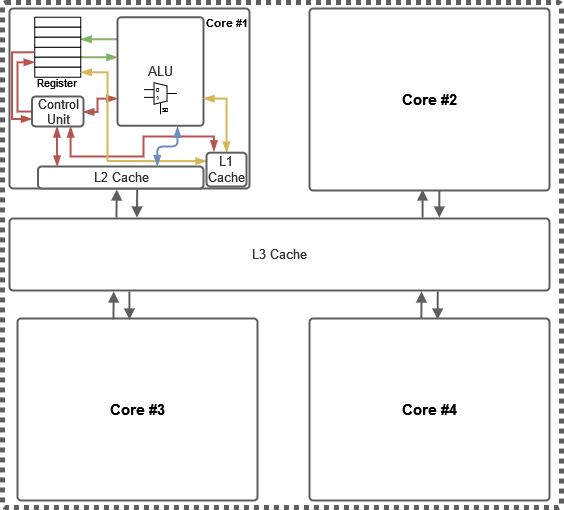
\includegraphics[width=0.7\linewidth]{Images/CPU.png}
\caption[Multi-Core CPU Architecture]{The CPU architecture consists of multiple cores, which contain components such as registers, caches, ALU and interconnects.}
\label{fig:CPU}
\end{figure} 
The CPU observed in \Fig{CPU} is an integrated circuit responsible for executing instructions and performing arithmetic, timing, logic and I/O operations. The CPU architecture involves the design and organisation of various components to optimise performance, power efficiency, and instruction execution. The main components are registers, arithmetic logic units (ALUs), control units, cache memory, and instruction pipelines. Registers are small, high-speed storage units within the CPU used for temporarily holding data and intermediate results during computation. ALUs are responsible for performing arithmetic and logic operations, such as addition, subtraction, NOT and OR. The control unit manages the flow of instructions and data within the CPU, fetching instructions from memory, decoding them, and coordinating their execution. CPU cache memory is used to store frequently accessed data, reducing the time taken to retrieve data from main memory.

Reduced Instruction (RISC) and Complex Instruction Set Computer (CISC) are two CPU microarchitecture approaches. RISC architectures prioritise simplicity and efficiency by employing a smaller set of basic instructions. This streamlined design typically leads to faster and more predictable execution, making RISC processors well-suited for power-constrained devices and applications where speed is critical. In contrast, CISC architectures, exemplified by x86, feature a diverse and extensive set of complex instructions designed to reduce the number of instructions required to perform tasks. While this complexity can provide convenience for programmers, it often results in more intricate hardware, potentially impacting performance and energy efficiency. 

Significant research is put into improving the execution speed of instruction pipelines. The pipeline breaks down the execution of instructions into multiple stages, allowing different instructions to be processed simultaneously. Each stage of the pipeline handles a specific task, such as instruction fetch, decode, execute, and write back. This pipelining process increases the CPU's instruction throughput and overall performance. CPU architecture also includes features like branch prediction, speculative execution, and out-of-order execution. Branch prediction predicts the outcome of conditional branches to keep the pipeline filled with useful instructions. Speculative execution allows the CPU to execute instructions before it is confirmed that they are needed, further improving performance. Out-of-order execution enables the CPU to execute instructions in a different order to optimise resource utilisation.

In the past decade, single-core processors have now been outpaced by the shift to multi-core designs. Traditionally, speedup was achieved by increasing the processor's clock speed and decreasing the transistor size to pack more into the silicon area. However, the power density required grew at a faster rate than the frequency which entailed power problems exacerbated by complex designs attempting to extract extra performance from the instruction stream. This led to designs that were complex, unmanageable, and power-hungry. However, chip designers introduced multiple cores onto a single die and leveraged parallel programming to continue pushing for more performance. The primary advantage to multi-core systems is the raw performance increase from extending the number of processing cores rather than clock frequency, which translates into slower growth in power consumption. This can be a significant factor in embedded devices that operate on a power budget, such as mobile devices. 

General-purpose multi-cores are becoming necessary in real-time digital signal processing. One general-purpose core would control various signals and watchdog functions for many special-purpose ASICS as part of a system-on-chip. This is primarily due to the variety of applications and functions required. Nevertheless, multi-Core processors give rise to new problems and challenges. As more processing cores are integrated into a single chip, power and temperature are the primary concerns that can increase exponentially with more cores. Memory and cache coherence is another challenge due to the distributed L1 caches and, in some cases, L2 caches which need to be coordinated.

%from these chips. Recent examples include image processing, audio processing, and wireless baseband processing. The computation behind these applications involves a sequence of operations processed on a stream of data that have little to no dependencies.
% Additionally, these operations can be performed in parallel and often require high throughput and performance to handle large amounts of data. Therefore, this favours designs with many processing elements that can compute these operations in parallel, improving power and performance.




\subsection{Graphics Processing Unit (GPU)}
%--------------------------------------------
\begin{figure*}[h]
\centering
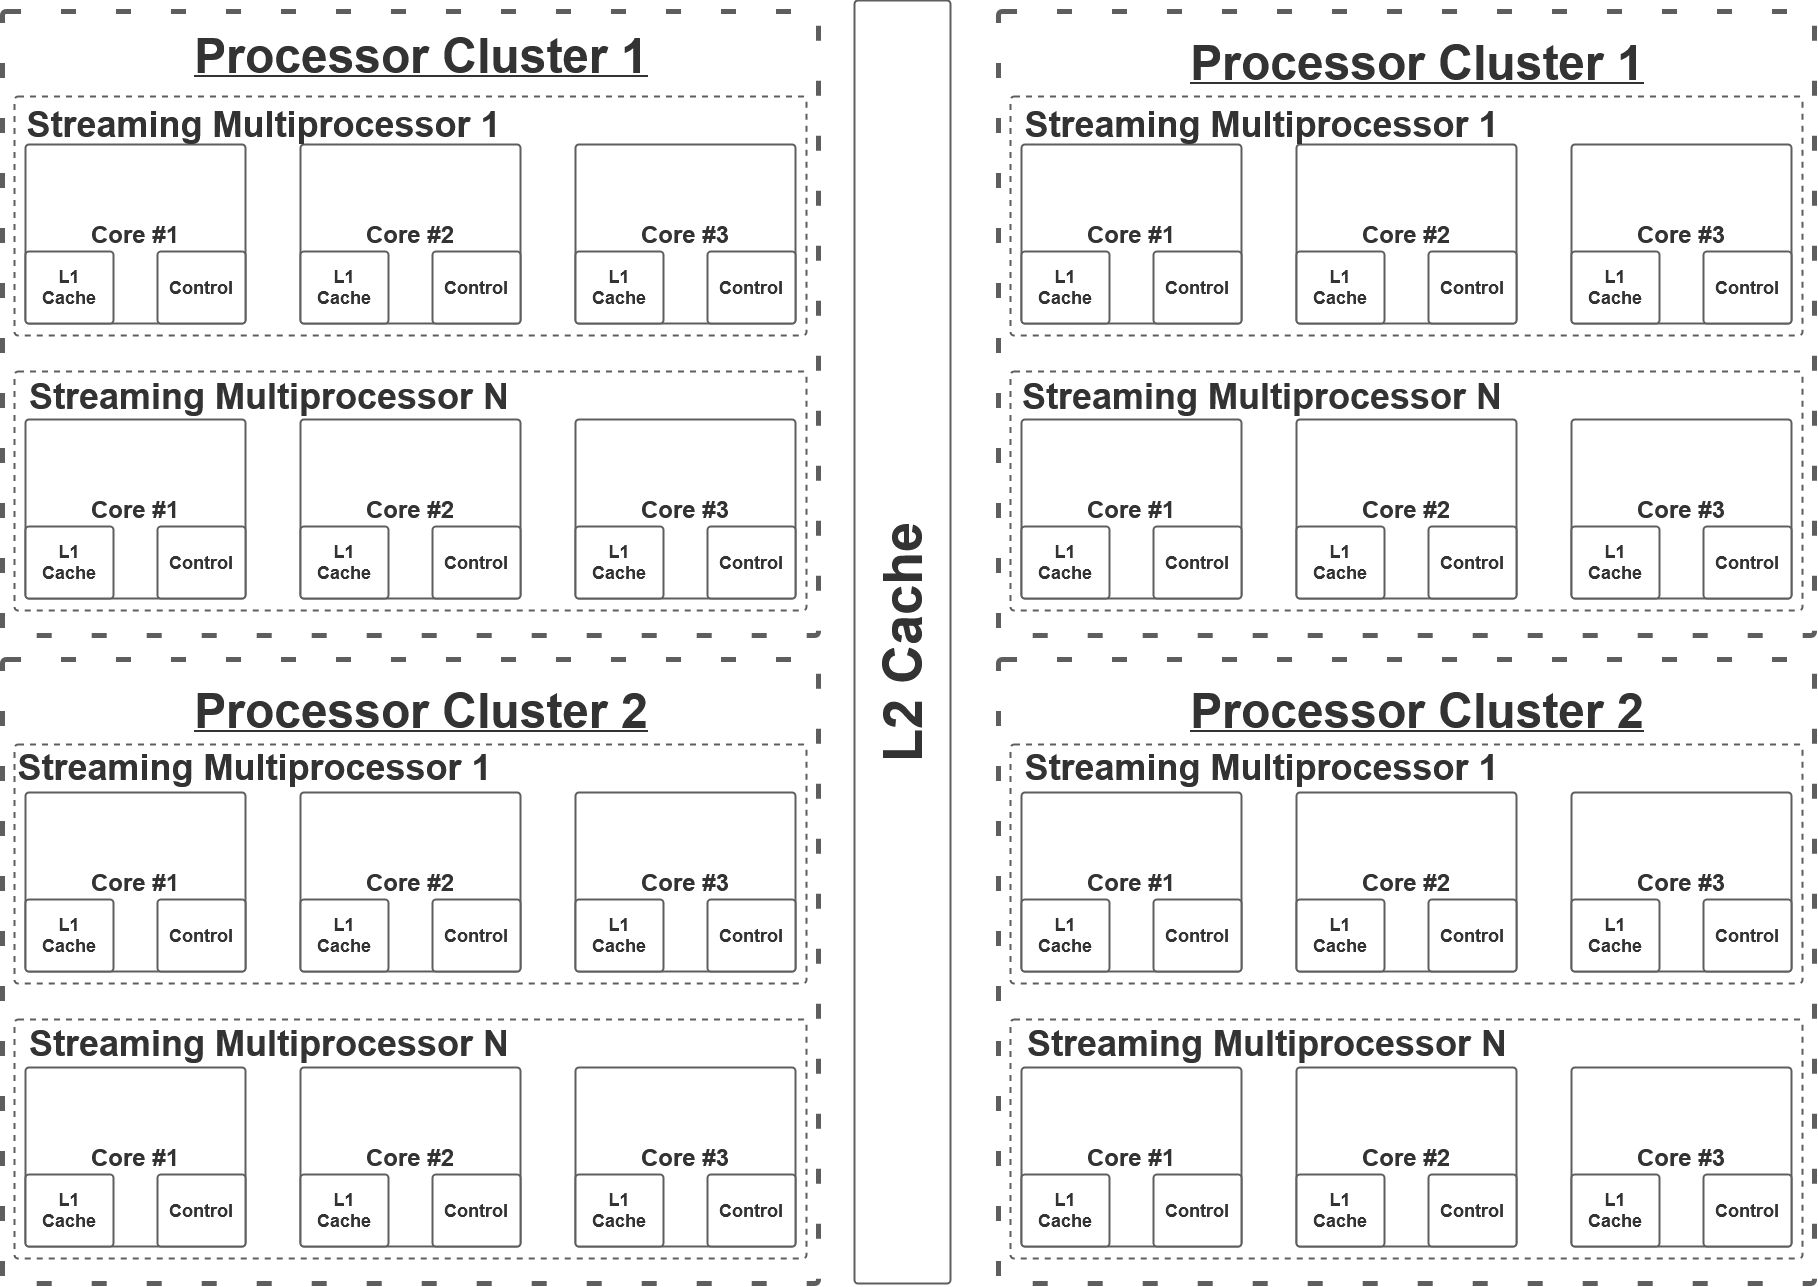
\includegraphics[width=\linewidth]{Images/GPU.png}
\caption[GPU Architecture]{ The GPU architecture comprises distinct elements, including Streaming Multiprocessors (SMs), Cache Hierarchy, and Compute Cores. SMs serve as the processing engines responsible for executing parallel threads, Cache Hierarchy optimises data access by efficiently managing on-chip memory caches, and Compute Cores perform complex computations and shader operations.}
\label{fig:GPU}
\end{figure*} 
%--------------------------------------------
The GPU is a specialised hardware architecture initially used for graphics rendering. However, GPUs have undergone significant power and cost advancements, which have captured the attention of both industry and academia. Designers have been exploring the potential of GPUs to accelerate large-scale computational workloads. 

The architecture of GPUs is designed with a focus on throughput optimisation, allowing for efficient parallel computation of numerous operations. \Fig{GPU} illustrates the high-level GPU architecture. The GPU comprises multiple Streaming Multiprocessors (SMs) that function independently, and these SMs are organised into multiple Processor Clusters (PCs). Each SM incorporates a layer-1 (L1) cache with each core. Typically, each SM possesses its dedicated layer-1 cache, and multiple SMs share a layer-2 cache before accessing data from the global GDDR-5 memory. Newer GPU models integrate tensor cores, which efficiently compute matrices calculations, enhancing their performance in deep learning tasks.

The GPU architecture, initially tailored for 3D graphics rendering, involves a streamlined pipeline with distinct stages. It commences with vertex processing, transforming 3D geometric data, followed by primitive assembly to group vertices into primitives. Rasterisation then translates these into screen pixels or fragments, and fragment processing adds attributes like colours and textures. Finally, the pixel output stage writes processed fragments to the frame buffer, resulting in the rendered image on the screen. The highly parallel nature of the graphics pipeline in GPUs makes them exceptionally well-suited for image processing tasks. Image processing often involves manipulating and analysing large amounts of pixel data concurrently, making it a naturally parallelisable task. Leveraging the parallel processing capabilities, image processing algorithms can be accelerated by providing higher frames per second performance for tasks such as image filtering, edge detection, and object recognition. Additionally, GPU optimised memory hierarchy ensures faster access and storage of larger images, kernels and intermediate data.

There remain drawbacks for GPUs, primarily if they are intended to be used as general-purpose machines. Firstly, the limitations of adaptability and context switching make them less suitable for general-purpose computing tasks. Simple calculations which do not utilise the parallelism are inhibited by lower clock speeds. Communication between the CPU and GPU can introduce bottlenecks and decrease the GPU throughput, especially when waiting for results from the CPU. Memory capacity and bandwidth would also affect GPU performance; for example, an image processing application must wait for the image data to be transferred from the main memory, further delaying the runtime. Lastly, GPUs cannot operate independently without support from a CPU, which contributes to more power consumption from idling. 

\subsection{Field-Programmable Gate Array (FPGA)}

\begin{figure*}[!ht]
\centering
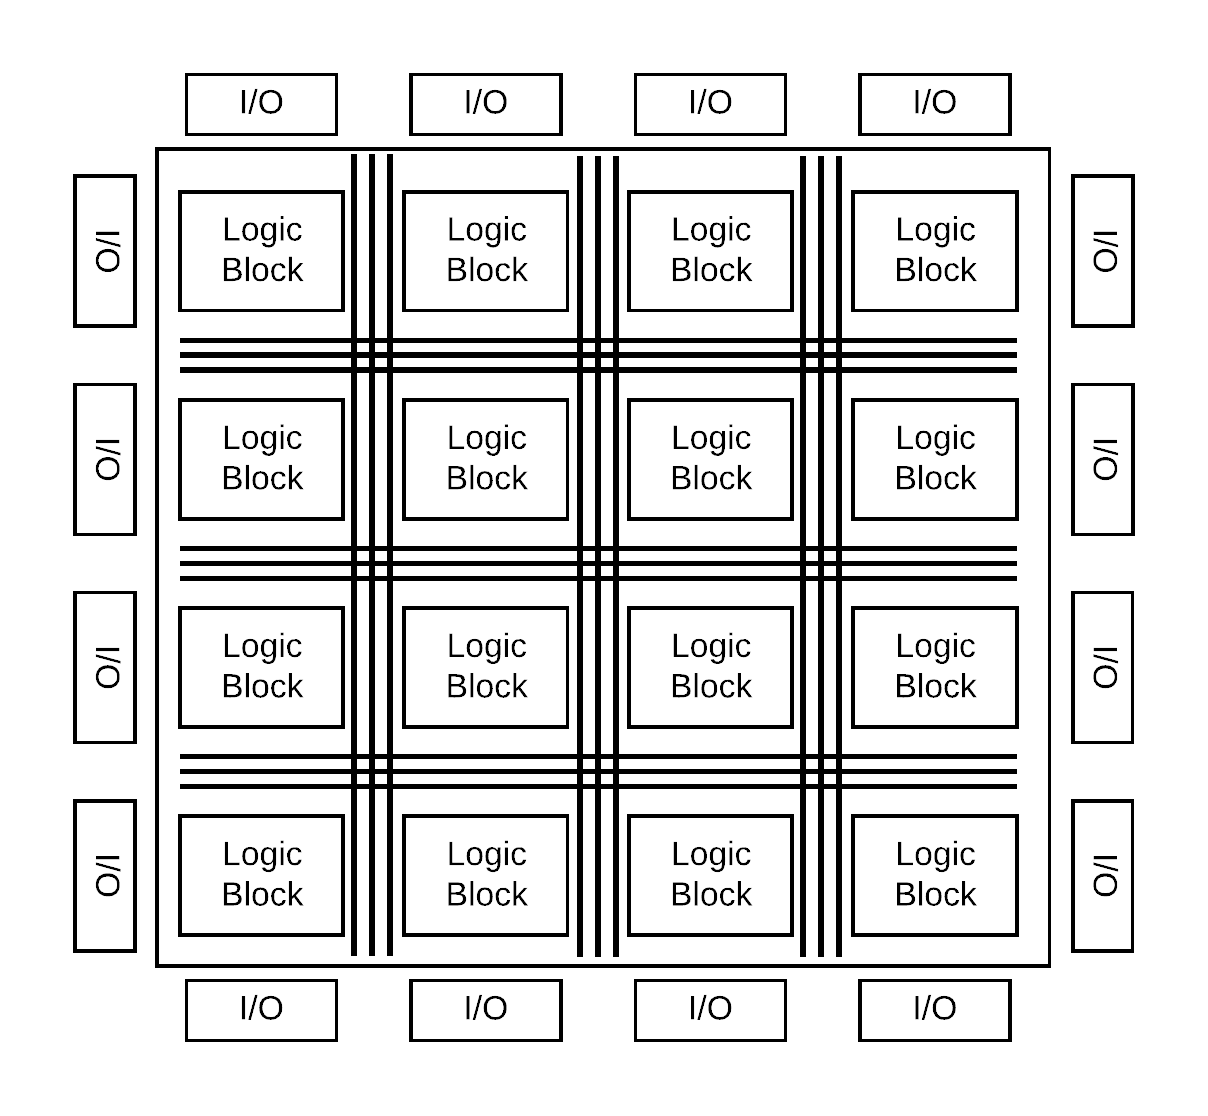
\includegraphics[width=0.7\linewidth]{Images/FPGA.png}
\caption[FPGA Architecture]{The FPGA Architecture contains Configurable Logic Blocks (CLBs), Interconnects, Programmable Routing, and I/O Resources components which define the Versatile and Reconfigurable Nature.}
\label{fig:FPGA}
\end{figure*} 

Field-Programmable Gate Arrays are versatile integrated circuits which offer direct hardware programmability for diverse applications. They have gained prominence due to their reconfigurability, making them highly advantageous compared to fixed processing architectures such as ASICs. These features enable shorter time-to-market by allowing prototyping and late-stage design modifications. The FPGA architecture, as depicted in \Fig{FPGA}, comprises a matrix of configurable logic blocks (CLBs) containing a combination of look-up tables (LUTs), shift registers (SRs), and multiplexers (MUXs). These components are interconnected through programmable high-bandwidth pathways and are surrounded by I/O ports.

The fine-grained nature of FPGAs empowers designers to exploit both spatial and temporal parallelism in their designs, resulting in enhanced performance. In image processing applications, algorithms can be tailored to operate on individual pixels or groups of pixels in parallel. Temporal parallelism can be achieved using techniques like pipelining, where separate processors work on successive stages of data, allowing concurrent processing and better throughput. Spatial parallelism, however, involves partitioning the image frame and processing each segment independently using separate processors.

FPGAs allow seamless integration of I/O, such as image sensors, enabling pixel data to be streamed directly into processing units without latency. Data can be routed efficiently to other embedded processors without external memory access. Block RAMs (BRAMs) within the FPGA enable exploiting data locality in vision kernels by keeping critical data on-chip. However, the main limitation in image processing applications often stems from external memory (E.g. DDR4 RAM) read/write operations, which can impact overall performance.

Advanced extensible interface (AXI) is a standard protocol for efficient communication between IP blocks within an FPGA design. It follows the Advanced Microcontroller Bus Architecture (ARM AMBA) specification, ensuring compatibility with ARM-based processors and systems-on-chip (SoCs). The AXI protocol supports separate read and write channels, enabling simultaneous data transactions in both directions. It also features burst transfers, allowing multiple data transfers within a single transaction to enhance data throughput.

Despite their advantages, FPGA development requires expertise in hardware descriptor languages (HDL), such as VHDL/Verilog. This steep learning curve can be a challenge for new developers accustomed high-level languages and instruction based architectures. In comparison to ASICs, the support functions and additional reconfigurable logic and power consumption overhead, making power efficiency considerations important during the design phase. FPGAs typically have limited on-chip memory compared to GPUs, which can have limitations for applications that require large memory spaces. Overall, FPGAs offer a powerful platform for image processing tasks, but their effective use requires careful consideration of design constraints and optimisation strategies.


\subsection{Application-Specific Integrated Circuits (ASICs)}
 ASICs are a specialised type of Very Large Scale Integration (VLSI) technology where integrated circuits are designed specifically for a particular application domain. This involves custom designing at the transistor level to optimise the circuit for performance and silicon area. There are several advantages of opting for an ASIC implementation over other general-purpose accelerators. The custom designed nature of ASIC logic allows designers to create tightly integrated applications, resulting in better performance, reduced power consumption, and minimised silicon usage. ASICs come with intrinsic trade-offs listed below:

\begin{itemize}
    \item \textbf{Fixed Design}: ASICs are designed for specific applications and lack flexibility compared to general-purpose processors. Once fabricated, it is challenging and costly to make modifications or upgrades to their functionality.
    \item \textbf{High Design Cost}: Designing and prototyping involves significant expertise and time, leading to higher initial development costs.
    \item \textbf{Long Development Timeline}: Creating a custom ASIC requires extensive expertise and significant time to design, verify, and manufacture. 
\end{itemize}

Despite these drawbacks, the per-chip manufacturing cost becomes significantly lower during mass production, rendering ASICs more economically viable for high-volume production. The following sections discuss the various types of ASICS targeting specific workloads:
 
\subsubsection{Vision Processing Units (VPUs)}
\begin{figure}[H]
\centering
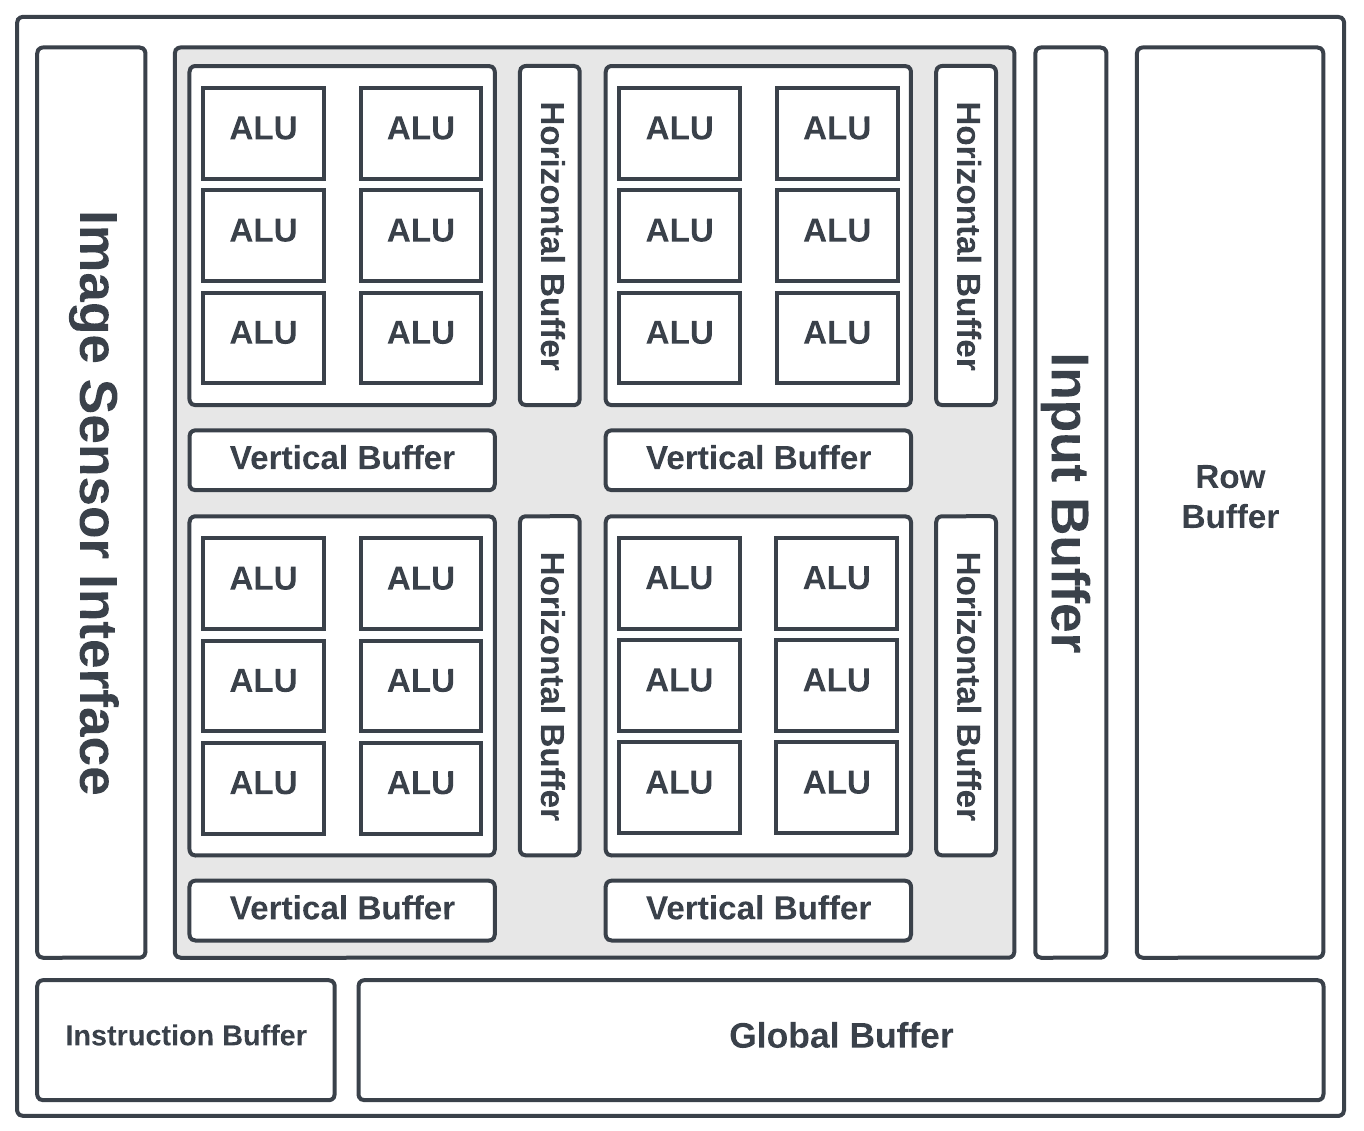
\includegraphics[width=10cm]{Images/VPU.png}
\caption[Vision Processing Unit Architecture]{VPU Architecture consists of an array of processing elements with horizontal and vertical buffers for efficient image processing.}
\label{fig:VPU}
\end{figure} 


VPUs are a class of ASIC designed to alleviate the heavy processing load on the central processor by accelerating workload-specific tasks. VPUs shown in \Fig{VPU} have a distinct hardware design that focuses on accelerating specific types of computations, such as deep learning inference, video encoding/decoding, and image processing. They often incorporate dedicated execution units, tensor cores, or specialised instructions to accelerate these tasks efficiently.

VPUs employ hardware architectures and software frameworks tailored to exploit parallelism and optimise performance for these tasks. GPUs, while also capable of accelerating AI workloads, are designed to handle a wide range of general-purpose graphics and compute tasks, making them more versatile but potentially less optimised for specific workloads.

VPUs also prioritise energy efficiency, aiming to deliver better performance per watt over other accelerators. They employ techniques like low-power execution units, reduced precision compute, and power management features to minimise energy consumption. GPUs, on the other hand, focus more on delivering absolute performance, often consuming more power in exchange for higher computational capabilities. In addition, VPUs often have specialised APIs or libraries that target specific applications or frameworks, enabling efficient execution of AI models or video codecs. However, the programming ecosystem for VPUs is limited in comparison to general-purpose architectures.

\subsubsection{Neural Processing Units (NPUs)}
 NPUs initially emerged in embedded devices as efficient AI inference accelerators specifically designed to manage the computational demands of machine learning workloads. The initial NPU architecture integrated high-density MAC arrays such as 2D GEMM or 3D systolic arrays since the majority of the computations are found within convolutional layers, which involve significant matrix multiplications. As CNNs continued to become increasingly complex with higher depth and many layers configurations, NPU has now optimised the MAC array structures to ensure enhanced modularity and scalability. Furthermore, newer features such as:

\begin{itemize}
    \item Fused operations
    \item Sparsity acceleration
    \item Unified High Bandwidth Memory
    \item Multi-level array partitioning
    \item Mixed Precision Support
\end{itemize}

NPUs have expanded their capabilities for other neural network architectures. This includes RNN/LSTM structures, targeting for audio and natural language processing, and transformers.


\subsubsection{Neuromorphic Hardware}
 Neuromorphic architectures are a type of hardware developed to mimic the structure and function of the human brain's neural networks. These architectures aim to replicate the principles of neural function in their operation, seeking inspiration from biological systems. By incorporating concepts such as weighted connections, activation thresholds, short and long-term potentiation, and inhibition, neuromorphic architectures aim to perform distributed computation in a way that resembles how the human brain processes information.

The key objective of neuromorphic architectures is to achieve efficient and parallel processing of data by leveraging the inherent capabilities of neural networks. These architectures often involve the use of spiking neural networks, where information is transmitted through spikes or pulses, similar to how neurons communicate in the brain. This approach allows for event-driven and energy-efficient computation, making neuromorphic architectures suitable for various tasks, including sensory data processing, pattern recognition, and complex decision-making. Despite their promising advantages, they face challenges, including complexity in design and implementation, limited applicability to specific tasks, scalability issues, lack of standardisation, and difficulty in implementing learning and adaptation mechanisms. Balancing energy efficiency and performance is another challenge, and commercial availability remains limited. 


\subsubsection{ASIC Summary}
\begin{table}[H]
\centering
\setlength{\extrarowheight}{0pt}
\addtolength{\extrarowheight}{\aboverulesep}
\addtolength{\extrarowheight}{\belowrulesep}
\setlength{\aboverulesep}{0pt}
\setlength{\belowrulesep}{0pt}
\caption{ASICs and Their Specifications}
\label{tab:ASIC_specs}
\resizebox{\linewidth}{!}{%
\begin{tabular}{lccccc} 
\toprule
\rowcolor[rgb]{0.753,0.753,0.753} \multicolumn{1}{c|}{\textbf{Manufacturer}} & \multicolumn{1}{c|}{\textbf{ASIC Type}} & \multicolumn{1}{c|}{\begin{tabular}[c]{@{}>{\cellcolor[rgb]{0.753,0.753,0.753}}c@{}}\textbf{Clock }\\\textbf{(MHz)}\end{tabular}} & \multicolumn{1}{c|}{\begin{tabular}[c]{@{}>{\cellcolor[rgb]{0.753,0.753,0.753}}c@{}}\textbf{Power }\\\textbf{(W)}\end{tabular}} & \multicolumn{1}{c|}{\begin{tabular}[c]{@{}>{\cellcolor[rgb]{0.753,0.753,0.753}}c@{}}\textbf{Process }\\\textbf{Node}\end{tabular}} & \textbf{Applications} \\ 
\midrule
Intel Movidius Myriad X & VPU & 1050 & 2.5 & 16nm & Edge devices, AI inference \\
Google TPU & TPU & 1800 & 10 & 7nm & Machine learning accelerators \\
ARM Ethos-U55 & NPU & 1000 & 1 & 7nm & IoT devices, edge computing \\
Huawei Kirin & NPU & 820 & 1 & 7nm & Smartphones, AI applications \\
Graphcore IPU & VPU & 500 & 252 & 16nm & AI workloads, data centres \\
Intel Neural Compute Stick & NPU & 700 & 1.5 & 28nm & Machine translation, NLP, Edge AI \\
\bottomrule
\end{tabular}
}
\end{table}

Table \ref{tab:ASIC_specs} offers a concise overview of various ASICS. These ASICs serve diverse purposes, from machine learning acceleration to edge computing and AI inference. Notable entries include the Intel Movidius Myriad X, known for its use in edge devices, and the Google TPU, a powerful tensor processing unit designed for machine learning tasks. The ARM Ethos-U55 and Huawei Kirin ASICs are optimised for IoT devices and smartphones, all while operating at low power consumption. Graphcore's IPU, on the other hand, stands out with its high power requirements, tailored for AI workloads in data centres. Lastly, the Intel Neural Compute Stick focuses on applications such as machine translation and natural language processing.

%--------------------------------------------------------

\subsection{Heterogeneous Architectures}

%-------------------------------------
\begin{figure}[H]
\centering
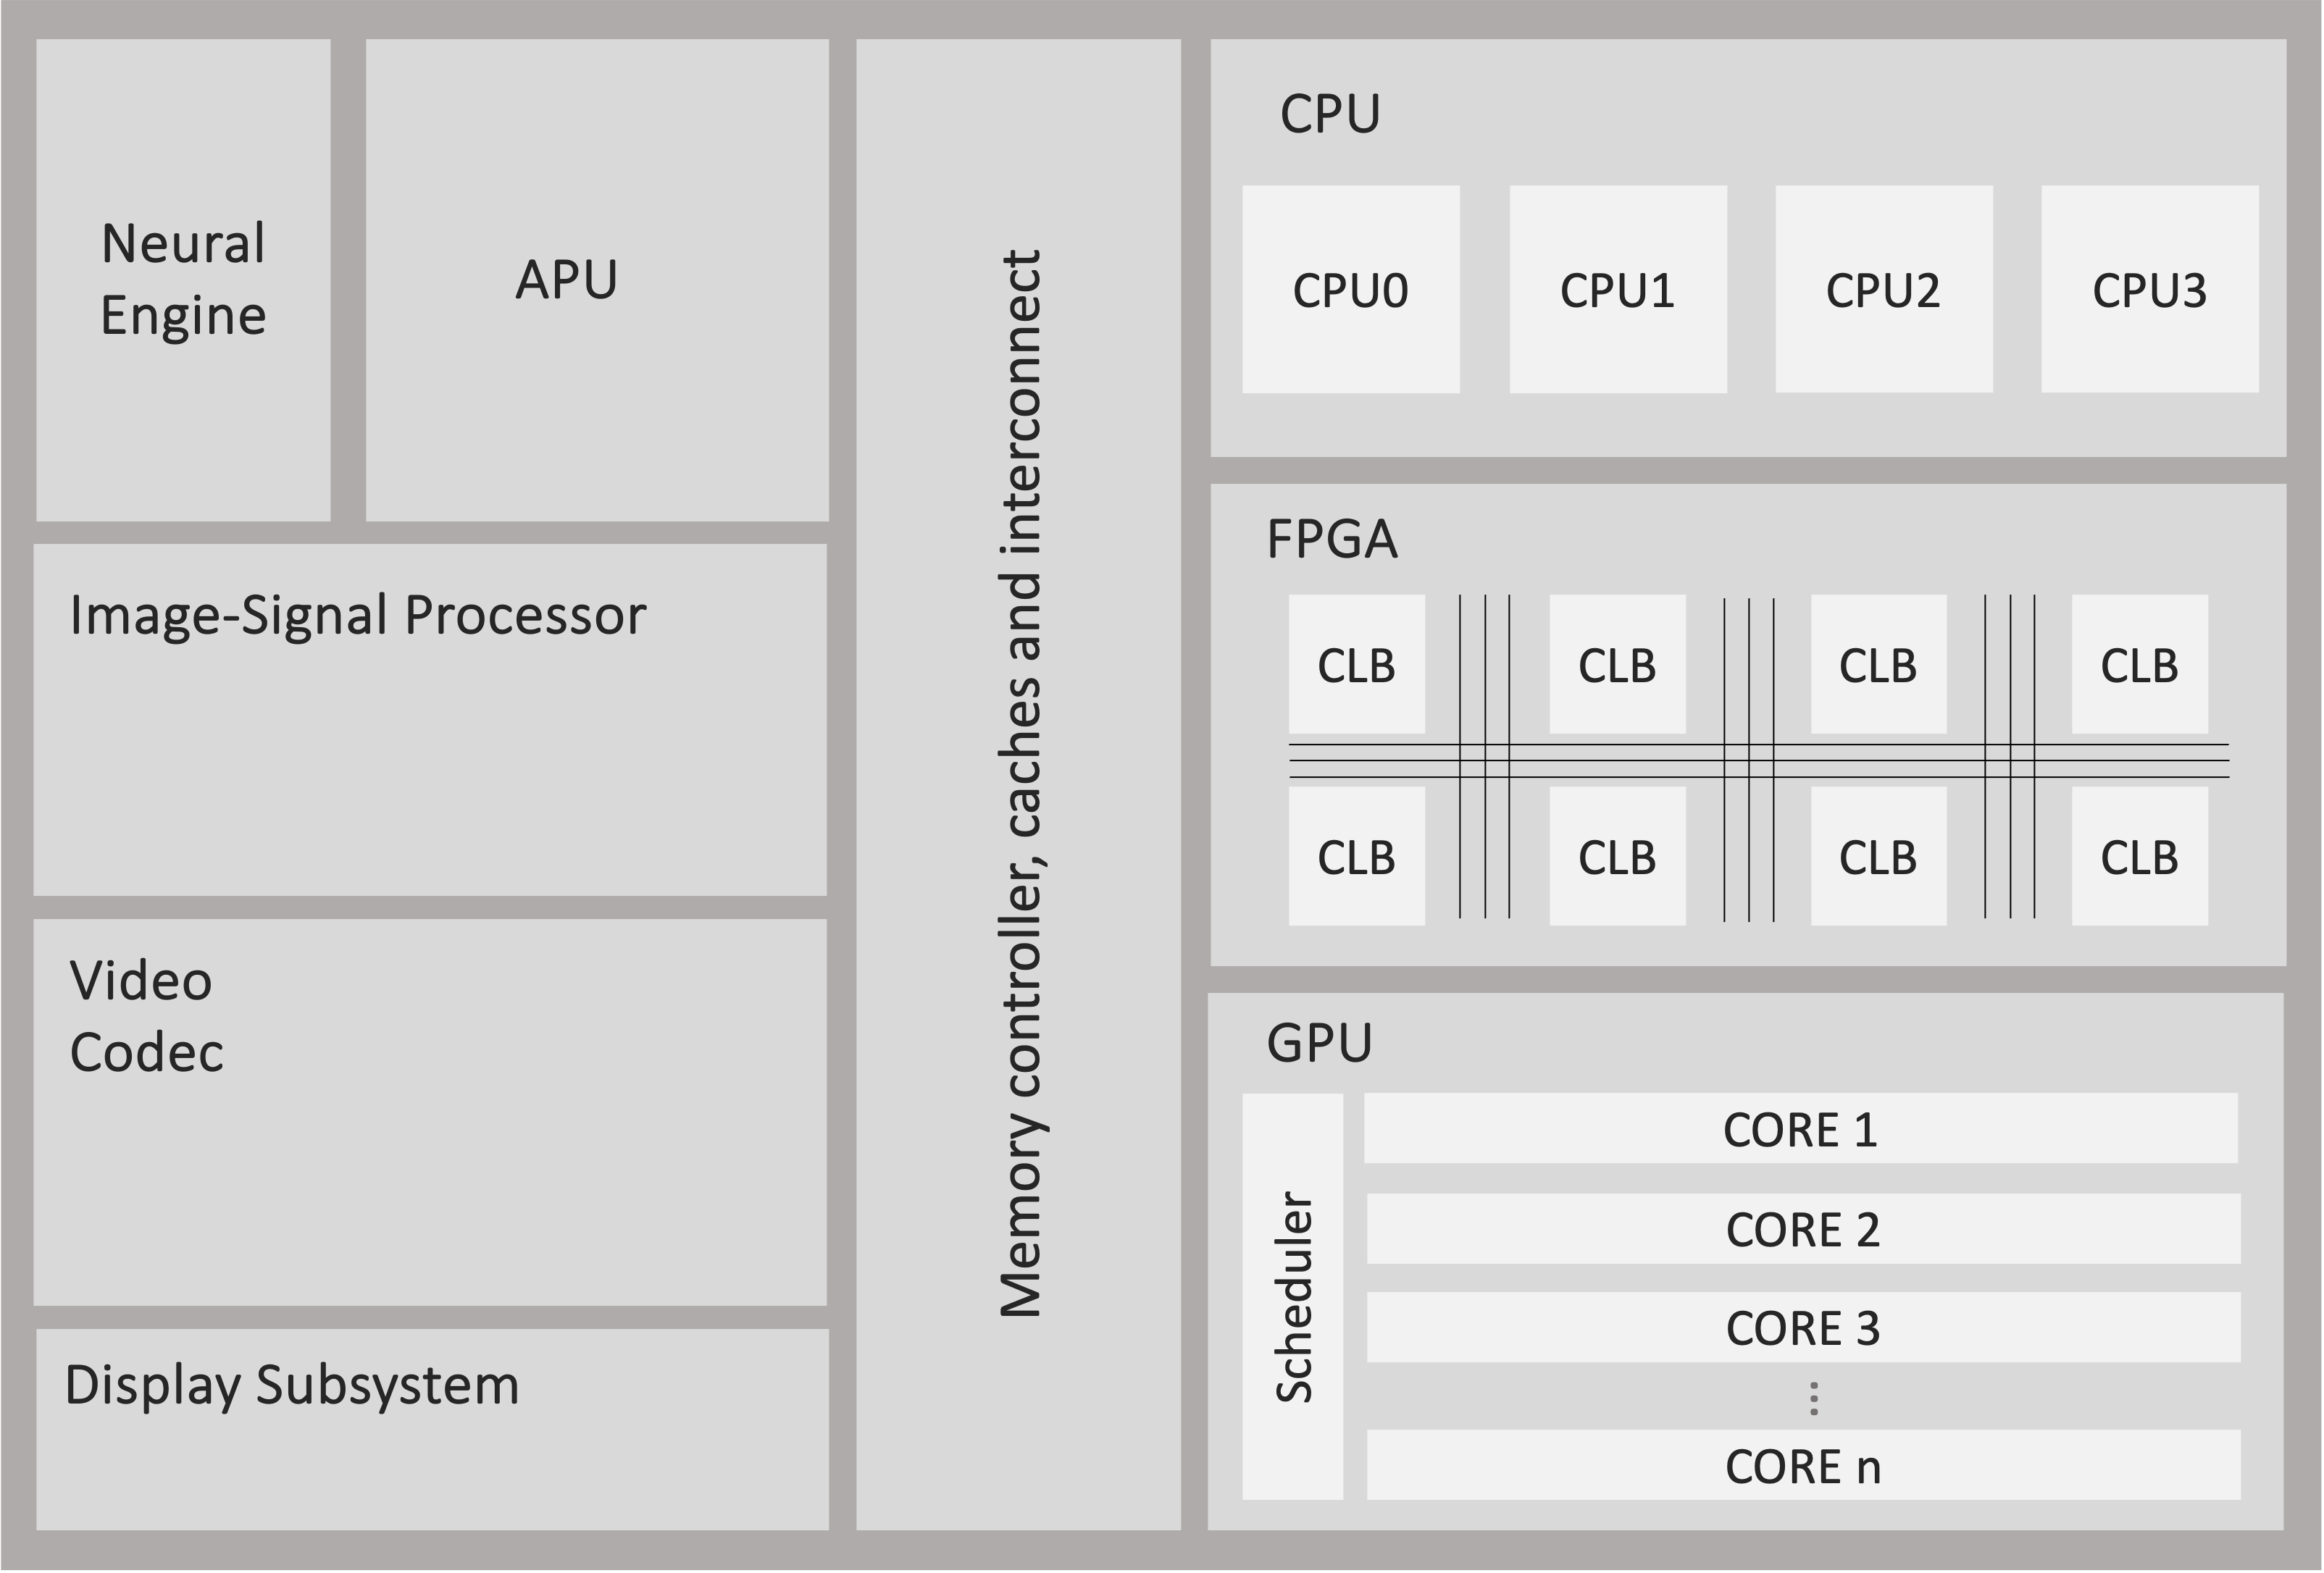
\includegraphics[width=11cm]{Images/Heterogenous.png}
\caption[Heterogeneous Architecture]{Concept Heterogeneous Architecture which integrate multiple specialised processing units onto a interconnected silicon chip. }
\label{fig:Heterogeneous}
\end{figure} 
%-------------------------------------
Heterogeneous architectures have recently gained significant attention and mainstream appeal in various application domains. These architectures integrate different types of accelerators, including CPUs, GPUs, NPUs, and FPGAs, into a single compute fabric, observed in \Fig{Heterogeneous}. Currently, commercial heterogeneous chips only contain a combination of CPU-GPU-NPU\cite{Intelhet}. The primary objective of heterogeneous architectures is to accelerate complex tasks by allocating specific operations to the most suitable specialised cores that can process them efficiently.

One of the key challenges in utilising heterogeneous systems lies in algorithm design. Designing algorithms that can effectively leverage the capabilities of different accelerators is crucial. It requires careful consideration of the characteristics and strengths of each accelerator, as well as the partitioning and mapping of computational tasks to the appropriate cores. Algorithm designers need to analyse the computational requirements, data dependencies, and parallelism inherent in the application to optimise the workload distribution across different cores.

Partitioning and mapping refer to the process of breaking down the computational tasks and mapping them onto the available cores. It involves considering the data dependencies, communication overhead, and resource utilisation to ensure efficient execution. Additionally, scheduling tasks across different cores, managing synchronisation between them, and optimising interconnect requirements are critical aspects of achieving optimal performance in heterogeneous architectures.

The programming environment for heterogeneous architectures can be complex and diverse. Each accelerator may have its own programming model, APIs, and language extensions, making it challenging to develop applications that can fully exploit the capabilities of all accelerators. Furthermore, the availability of libraries and software tools may vary across different compute elements due to differences in instruction set architectures. This can lead to binary incompatibility and limit the portability of applications across different accelerators. Evaluating the performance of heterogeneous architectures requires comprehensive performance evaluation techniques. Benchmarks and performance metrics need to consider the characteristics of the application, workload distribution, and communication patterns to provide an accurate assessment of the system's capabilities.


\subsection{Summary}
\begin{table}[H]
\centering
\setlength{\extrarowheight}{0pt}
\addtolength{\extrarowheight}{\aboverulesep}
\addtolength{\extrarowheight}{\belowrulesep}
\setlength{\aboverulesep}{0pt}
\setlength{\belowrulesep}{0pt}
\caption{Hardware Architecture Specification Summary.}
\label{tab:HardwareSummary}
\arrayrulecolor{black}
\resizebox{\linewidth}{!}{%
\begin{tabular}{c|c|c|c|c|c|c} 
\toprule
\rowcolor[rgb]{0.753,0.753,0.753} {\cellcolor[rgb]{0.753,0.753,0.753}} & {\cellcolor[rgb]{0.753,0.753,0.753}} & \multicolumn{2}{c|}{Compute Type} & {\cellcolor[rgb]{0.753,0.753,0.753}} & \multicolumn{2}{c}{Execution Paradigm} \\ 
\hhline{>{\arrayrulecolor[rgb]{0.753,0.753,0.753}}->{\arrayrulecolor{black}}|>{\arrayrulecolor[rgb]{0.753,0.753,0.753}}->{\arrayrulecolor{black}}|-|-|>{\arrayrulecolor[rgb]{0.753,0.753,0.753}}->{\arrayrulecolor{black}}|-|-}
\rowcolor[rgb]{0.753,0.753,0.753} \multirow{-2}{*}{{\cellcolor[rgb]{0.753,0.753,0.753}}Architecture} & \multirow{-2}{*}{{\cellcolor[rgb]{0.753,0.753,0.753}}Flexibility} & Temporal & Spatial & \multirow{-2}{*}{{\cellcolor[rgb]{0.753,0.753,0.753}}Latency} & Dataflow & Instruction \\ 
\cmidrule{1-4}\cline{5-5}\cmidrule{6-7}
CPU & General & \checkmark & \checkmark & Medium & × & \checkmark \\ 
\midrule
GPU & General & \checkmark & \checkmark & High & × & \checkmark \\ 
\midrule
FPGA & General & ~ ×\textsuperscript{(1)} & \checkmark & Low & \checkmark & × \\ 
\midrule
ASIC & Fixed & × & \checkmark & Low & \checkmark & × \\
\bottomrule
\multicolumn{7}{c}{(1) FPGA's can support temporal compute, however impractical considering overhead and effectiveness.} \\
\end{tabular}
}
\end{table}
The table \ref{tab:HardwareSummary} provides a concise overview of various hardware architectures used in compute operations. CPUs and GPUs offer general-purpose flexibility, supporting temporal and spatial computations with medium and high latency, respectively, while following an instruction-based execution paradigm. FPGAs, though generally flexible, are better suited for spatial computations, with limited practicality for temporal tasks due to overhead and effectiveness constraints. They employ a dataflow execution paradigm. In contrast, ASICs are fixed-function hardware designed for specific spatial computations, offering low latency and following a dataflow execution paradigm.

\subsection{Software Ecosystem}
This section explores the software domain employed for targeting hardware architectures and software interfaces. Optimised libraries such as OpenCV, High-Level Synthesis, and Domain-Specific Languages assume a role in bridging the gap between hardware and software application development.

\subsubsection{High-Level Synthesis (HLS)}
High-level synthesis (HLS) is a tool that enables hardware designers to use a high-level programming language, such as Python, C or C++, to create hardware designs. This is in contrast to traditional hardware design methods, which involve manually writing hardware description languages (HDLs) such as VHDL or Verilog. HLS tools take in the high-level source code and automatically generate the corresponding HDL code. This can greatly simplify the design process, making it more accessible to non-hardware design experts. This means that designers can focus on the functionality of the design and not worry about low-level implementation details. HLS tools also perform optimisation to improve the performance and resource utilisation of the generated hardware. This can result in more efficient designs that use fewer resources and run faster.

% HLS is widely used in the development of digital signal processing, computer vision, and machine learning algorithms. These types of applications are often complex and require a high level of parallelism, making them well-suited for implementation in hardware. HLS can also be used for hardware verification, which is the process of ensuring that the generated hardware behaves as expected. This can be done through co-simulation, where the generated hardware is simulated alongside the software to check for correct behavior.

Another benefit of HLS is that it allows for faster design iteration. As the design can be expressed in a high-level programming language, it can be easily modified and re-synthesised to see the effects of the changes. This can greatly speed up the design process and allow for faster time-to-market. In addition, FPGAs are often selected for systems where time to market is critical in order to avoid lengthy chip design and manufacturing cycles. The designer may accept the increased performance, power, or cost in order to reduce design time. Modern HLS tools put this trade-off into the hands of the designer; with more effort, the quality of the result is comparable to handwritten RTL (register transfer language). ASICs have high manufacturing costs, so there is a lot of pressure for designers to achieve success on the first attempt. Design iterations can quickly and inexpensively be done without huge manufacturing costs.

% The design effort of FPGA implementations in hardware description languages remains high. HLS was first proposed in the 1980s, but recently a renewed interest formed within recent years, notably as a design methodology for field-programmable gate arrays (FPGAs). While FPGA design has historically been only developed by hardware engineers, HLS offers a path to allow the ability to work at a higher level of abstraction by using C/C++ to specify the hardware functionality. This allows software developers to implement designs on FPGA to exploit its benefits of higher throughput and energy efficiency relative to standard processors.

% The HLS step includes, firstly, allocating necessary
% resources for the computations needed in the provided behavioural description (Allocation stage). Secondly, the allocated resources are bound to the corresponding operations (Binding stage). Thirdly, the operations order of execution is scheduled (Scheduling stage). The output of the high-level synthesiser is an RT-level description. The RT-level description is
% then logically synthesised to produce an optimised netlist. Gate netlists are then converted into circuit modules by placing cells of physical elements (Transistors) into several rows and connecting input/output (I/O) pins through routing in the channels between the cells. The following example illustrates the HLS stages (Allocation, Binding, and Scheduling).

However, these tools come with a set of drawbacks. For instance, the initial learning curve can be steep, particularly for those new to hardware design, as they require a solid understanding of both high-level programming and hardware optimisation techniques. While HLS tools automate the allocation of hardware resources based on the provided code, they may not always yield the most efficient designs for complex projects compared to manual, fine-tuned hardware descriptions. One of the key challenges in using HLS tools is accurately predicting the performance of the generated hardware. Factors such as memory access patterns, data dependencies, and the overall architecture can significantly impact performance, making it challenging to estimate how the synthesised hardware will behave. Moreover, debugging HLS-generated designs can be complex. Traditional software debugging methods are often insufficient, as hardware-related issues might not manifest in the same way as in software. This can prolong development cycles and hinder the identification of issues.

% Hardware synthesis is a general term used to refer to the processes involved in
% automatically generating a hardware design from its specification. High-level Synthesis (HLS) could be defined as the translation from a behavioural description of the intended hardware circuit into a structural description similar to the compilation of programming languages (such as, C, Pascal, etc.) into assembly language. The behavioural description represents an algorithm, equation, etc., while a structural description represents the hardware components that implement the behavioural description. In spite of the general similarity between hardware and software compilations, hardware synthesis is a multi-level and complicated task. In software compilation, you translate from a high-level language to a lower-level language, while in hardware synthesis you step through a series of levels.


% A study by NEC \cite{Kaz04} describes the benefits of HLS tools raising the abstraction level. The paper shows that a 1M-gate design typically requires about 300k lines of RTL code which cannot be easily handled by a human designer. The code density can be reduced by 7x to 10x when using a high-level specification in C, C++. The same 1M-gate design can be described into 40k lines of behavioural description, therefore reducing design complexity. Another advantage of HLS tools is that FPGA's are often selected for systems where time to market is critical in order to avoid lengthy chip design and manufacturing cycles. The designer may accept the increased performance, power, or cost in order to reduce design time. Modern HLS tools put this trade-off into the hands of the designer; with more effort, the quality of the result is comparable to handwritten RTL (register transfer language). ASIC's have high manufacturing costs, so there is a lot of pressure for designers to achieve success on the first attempt. Design iterations can quickly and inexpensively be done without huge manufacturing costs.

\subsubsection{Domain-Specific Languages (DSL)}
Domain-specific languages (DSLs) are programming languages designed to address specific problem domains rather than being general-purpose languages. DSLs offer higher-level abstractions and syntax tailored to a particular application area, allowing users to express domain-specific concepts more concisely and intuitively. Unlike general-purpose languages, DSLs enable non-experts to work effectively within a specific domain, as they are more focused on the domain's requirements and semantics. DSLs come in two main types: external DSLs, which are standalone languages distinct from the host language  (\eg Cal Actor Language\cite{Eker}), and internal DSLs, which are embedded within a general-purpose language using its syntax and tools (\eg Halide \cite{10.1145/2491956.2462176}). The use of DSLs can lead to improved productivity, reduced error rates, and better code maintainability in specific application areas.

\subsubsection{Libraries \& Frameworks}
Optimised libraries such as OpenCV\cite{opencv_library} are essential tools used to develop vision and deep-learning applications. These libraries offer a comprehensive collection of pre-built algorithms and functions for a wide range of image-related tasks. Their significance lies in the substantial time and resource savings they provide, enabling developers to utilise tried-and-tested algorithms, thus reducing development efforts and benefiting from community-driven improvements. Moreover, optimised libraries ensure cross platform compatibility, supporting various programming languages and platforms. They are continually updated to harness advancements in hardware and software, making them key for efficient and adaptable image processing.

Deep learning frameworks such as Pytorch\cite{Pytorch} offer abstraction and simplification, allowing developers to focus on high-level tasks. Frameworks encompass a comprehensive suite of support programs, compilers, code librar-ies, toolsets, and application programming interfaces that provide a cohesive environment that streamlines the development of systems. Therefore, frameworks facilitate rapid prototyping and integration with other tools.

\section{Conclusion}
In conclusion, this section provides an in-depth overview of the imaging pipe-line and its fundamental components, establishing the groundwork for the subsequent chapters. It encompasses typical operations present in each pipeline stage, which will used as implementation examples. Furthermore, the section delves into diverse hardware platforms such as CPUs, GPUs, VPUs, and FPGAs, each offering distinct attributes that can accelerate algorithms. To leverage these hardware capabilities, a range of tools and methodologies are introduced, which include high-level synthesis. In the next chapter, the state-of-the-art study on heterogeneous architectures and optimisation strategies related to image processing are discussed.